
\section{TJ-Monopix1 characterization}
    \subsection{Front end parameters}


    \subsection{Threshold and noise: figure of merit for pixel detectors}
        %python3 -i calibration/scurve_tot_histo.py -f calibration/calibration_data/20220506 -i 1 100 questo script crea i file di output contenenti i gli istogrammi del tot e della s curve
        %python3 -i calibration/tot_charge_plotting.py -f calibration/calibration_data/20220506 per fare il plot della s curve e relativi residui 
        %python3 -i calibration/tot_histo2d.py -f calibration/calibration_data/PMOS/20220506 per fare l'istogramma 2d del tot
        \begin{figure}[h!]
            \centering
            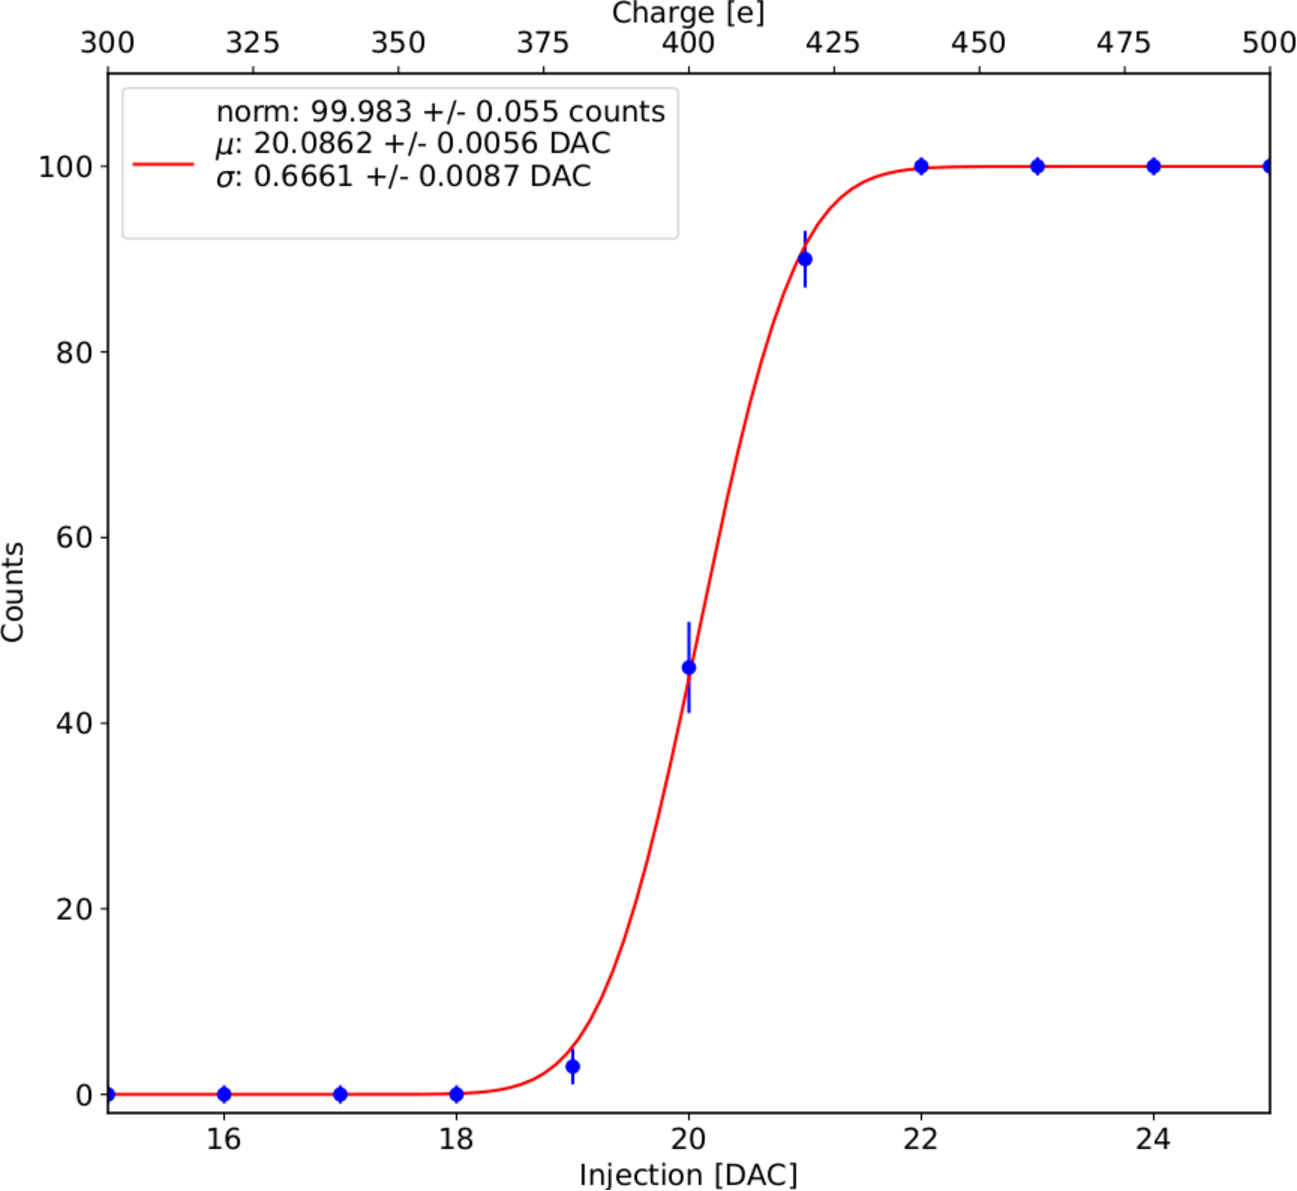
\includegraphics[width=.6\linewidth]{figures/charaterization/scurve.pdf}
            \caption{S curve for pixel (10, 10) of the PMOS flavor. The conversion of charge injected from DAC to electrons has been done assuming a conversion factor of \SI{20}{e-/DAC}.}
            \label{fig:scurve}
        \end{figure}   

        \begin{figure}[h!]
                -\begin{subfigure}{.5\textwidth}
                \centering
                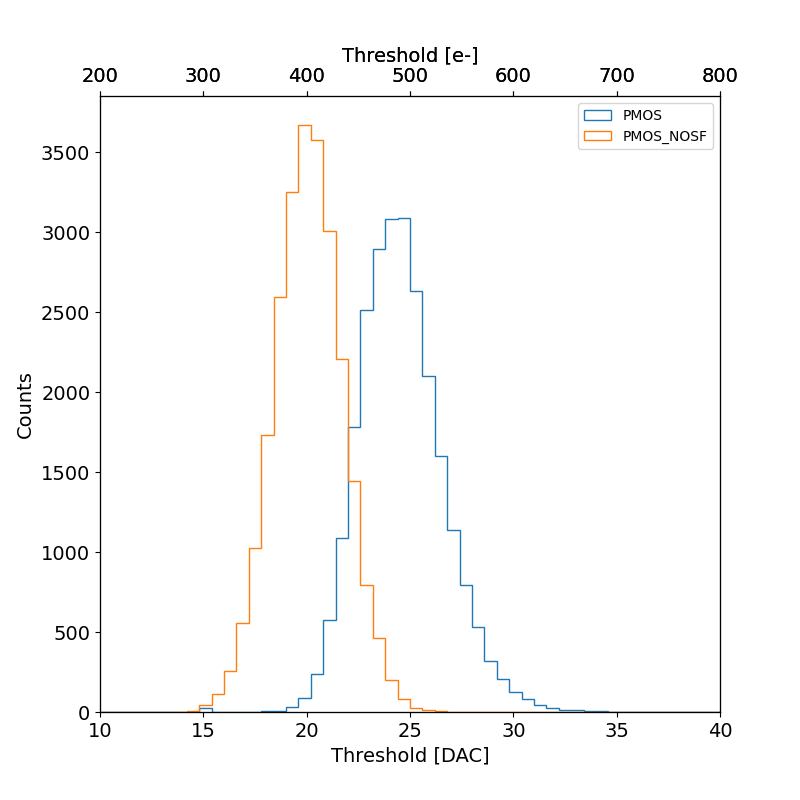
\includegraphics[width=.99\linewidth]{figures/charaterization/threshold_histogram.png}
                \caption{}
                \label{fig:}
                \end{subfigure}
                \begin{subfigure}{.5\textwidth}
                \centering
                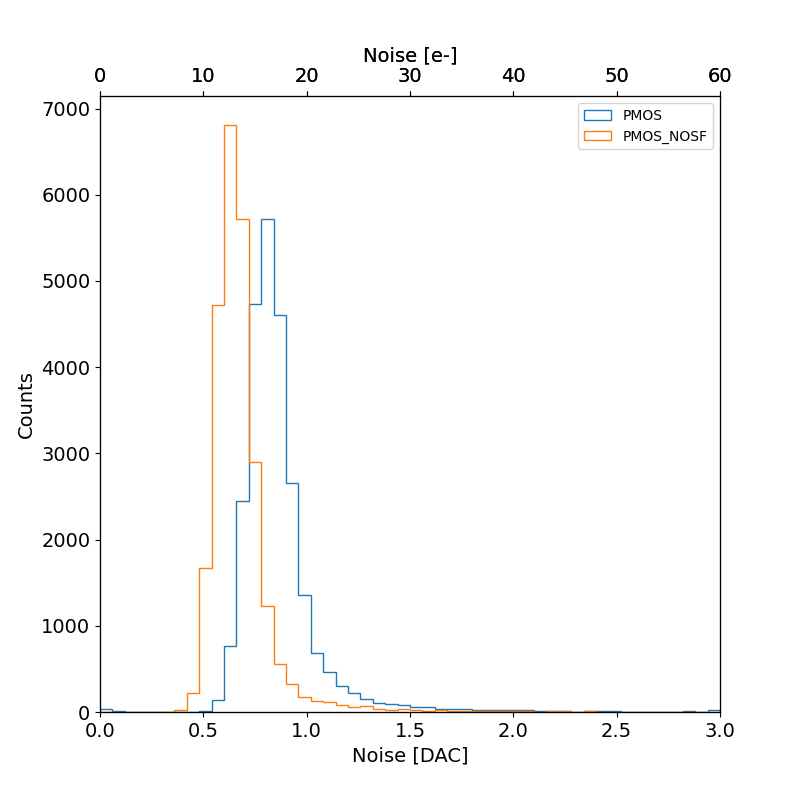
\includegraphics[width=.99\linewidth]{figures/charaterization/noise_histogram.png}
                \caption{}
                \label{fig:threshold_noise_hist}
                \end{subfigure}
        \end{figure}            
           
        \begin{figure}[h!]
            \begin{subfigure}{.5\textwidth}
            \centering
            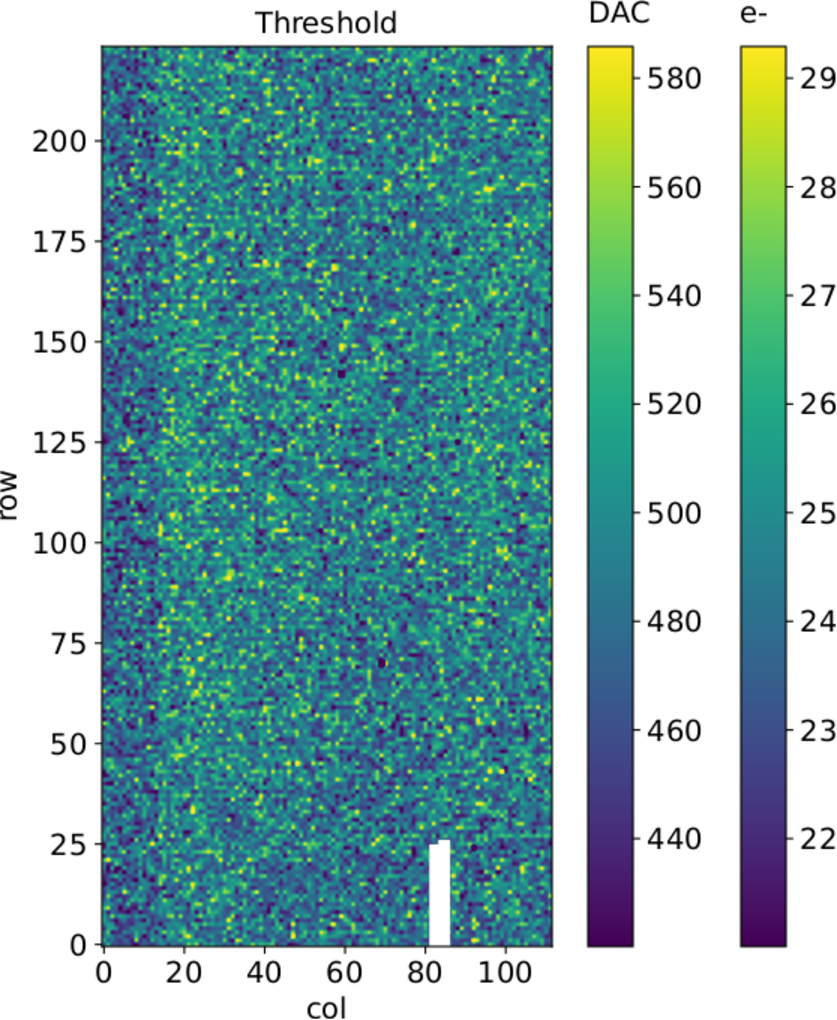
\includegraphics[width=.99\linewidth]{figures/charaterization/threshold_map.pdf}
            \label{fig:}
            \end{subfigure}
            \begin{subfigure}{.5\textwidth}
            \centering
            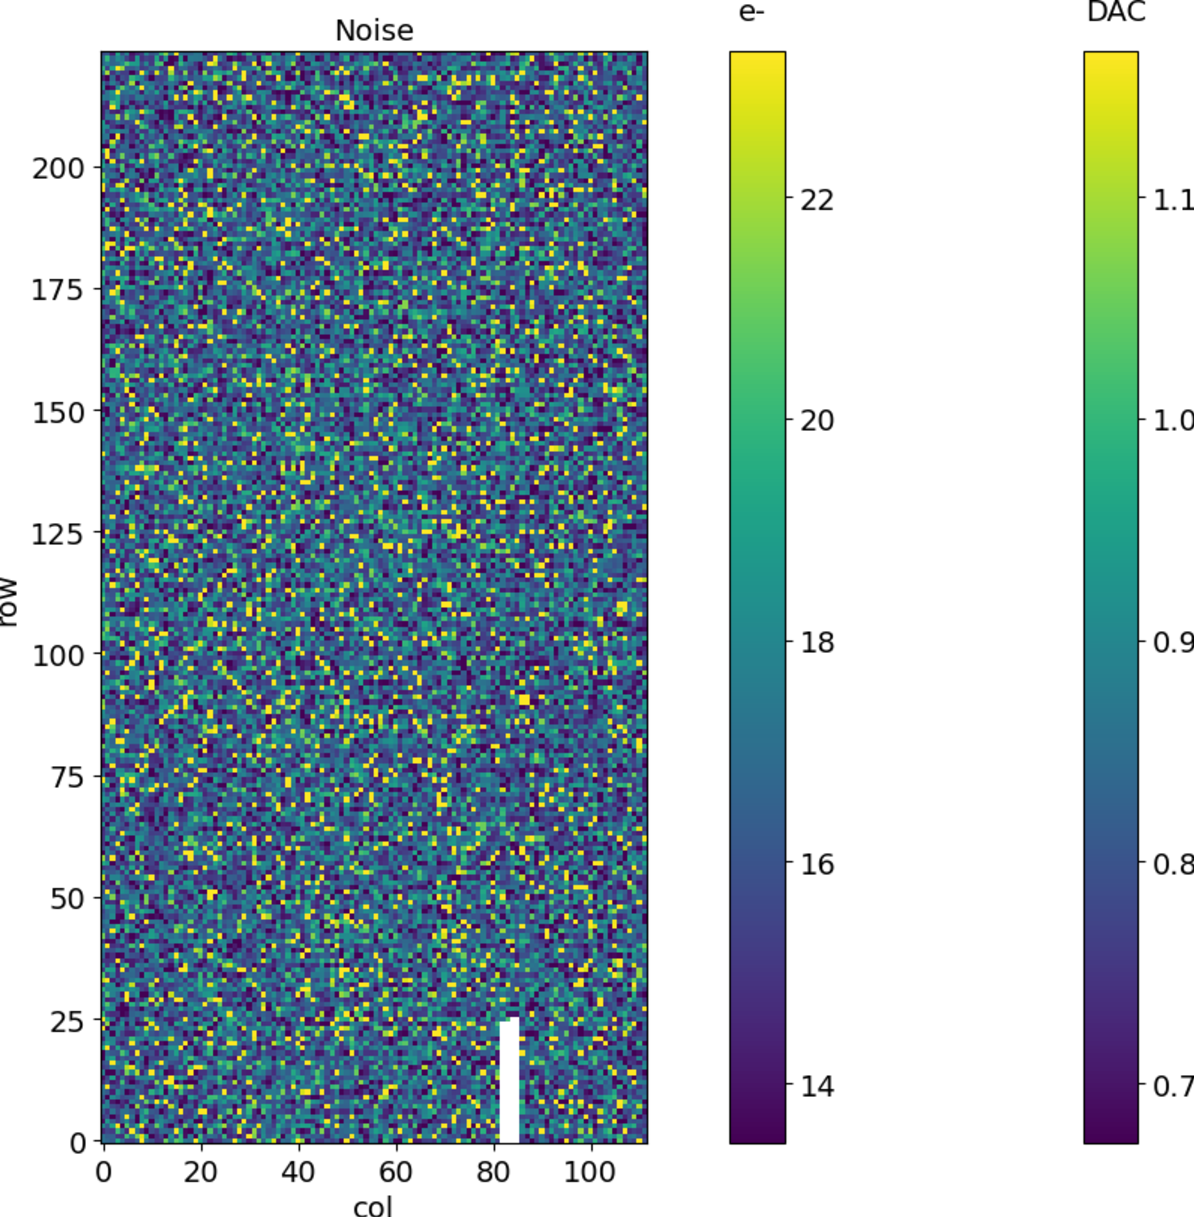
\includegraphics[width=.99\linewidth]{figures/charaterization/noise_map.pdf}
            \label{fig:threshold_noise_map}
            \end{subfigure}
            \caption{}
        \end{figure} 
        
        \red{Una caratterizzazione di soglia e rumore è necessaria in quanto questi valori condizionano sia le condizioni di operatività di questi chip, che le performance. }
        infact, the signal to threshold ratio may be considered as the figure of merit for pixel detectors rather than the signal to noise ratio.
        The mean minimum stable threshold evolved through different generation of chips: in the 1st generation it was around \SI{2500}{e-} while in the 3rd (corresponding to nowadays chips) is less than \SI{500}{e-}. This allows in thinner sensors with smaller signals: from \SI{16000}{e-} produced in \SI{200}{\um}, the signal expected moved down to \SI{2000}{e-} produced in \SI{25}{\um}. According with this \red{??}, the threshold of TJ-Monopix1 is around \SI{500}{e-}.
        \red{The following prototypes hanno una soglia e un rumore più bassi, ad esempio TJ-Monopix2 ha una soglia e un rumore... }
        The threshold has to be located between the noise peak around the baseline and the signal distribution, in particular it has to be low enough to mantain a high signal efficiency, but also high enough to cut the noise: for a low threshold many pixels can fire at the same time and a positive feedback can set off a chain reaction eventually, causing all the other pixels to fire.
        \red{Thus, the noise sets a lower bound to the threshold: if an occupancy $\leqslant$ $10^{-4}$ is required, for example, this correspond to the Gaussian 1-sided tail fraction for \SI{3.7}{\sigma}.
        In this case, if the noise is \SI{100}{e-}, for example, the threshold must be higher than \SI[parse-numbers=false]{3.7\times100}{e-}.}
        Typically this argument sets only a minimal bound to the threshold since the variation with time and from pixel to pixel have to be taken into account: the temperature, the anealing (for example, the radiation damages in the oxide layer causes shift of MOSFET threshold voltage) and the process parameters variation across the wafer (as for example process mismatch between transistors). 
        
        On the other hand the noise is valued at the preamplifier input node given that the first stage of amplification is the most crucial since the signal amplitude is high compared to additional noise introduced by the following stages.
        The noise is then parameterized as Equivalent Noise Charge (ENC), which is defined as the ratio between the noise N at the output expressed in V and the out voltage signal S produced by \SI{1}{e-} entering in the preamplifier:
        \begin{equation}
            ENC\, =\, \frac{N_{out}[V]}{S_{out}[V/e-]}\,=\,\frac{V^{RMS} _{noise}}{G}
        \end{equation} 
        with G expressed in \si{V/e-}.
        As the gain increases, the noise reduces (\red{da testare: fai uno scan}). 

        ENC is mainly influenced by the total input capacitance and by the system bandwidth: if the bandwidth is constant, noise can be reduced by increasing the input transistor transconductance (and consequently power consumption). \red{da capire meglio}
        Considering the threshold dispersion a requirement for the ENC is: 
        \begin{equation}
            ENC < \sqrt{(T/3.7)^2 - T_{RMS} ^2 (x) - T_{RMS} ^2 (t)}
        \end{equation}
        where the T is the threshold set, $T_{RMS}$ is the threshold variation during time (t) and across the matrix (x); a typical reasonable value often chosen is \SI{5}{ENC}.

        Because of the changing of the 'real' threshold, the possibility of changing and adapting the setting parameters of the FE, both in time and in space is desiderable: these parameters are usually set by Digital to Analog Converter (DAC) with a number of bit in a typical range of 3-7.
        Unfortunately DAC elements require a lot of space that may be not enough on the pixel area; therefore, the FE parameters are typically global, which means that they are assigned for the whole chip, or they can be assigned for regions the matrix is divided into. 
        The former case corresponds to TJ-Monopix1's design in which 7 bits are used for a total 127-DAC possible values, while the latter corresponds to the ARCADIA-MD1's one, \red{where quanti bit??}. 
        An other possibility, for example implemented in TJ-Monopix2, is allocate the space on each pixel for a subset of bits, then combinig the global threshold with a fine tuning. 
        If so, the threshold dispersion after tuning is expected to be inversely proportional to the tuning DAC number of bits:
        \begin{equation}
            \sigma_{THR, tuned} = \frac{\sigma_{THR}}{2^{n bit}}
        \end{equation}    
        where $\sigma_{thr}$ is the RMS of the threshold spread before tuning.

        To measure the threshold and noise of pixels a possible way is a scan with different known injected charge: the threshold corresponds to the value where the efficiency of the signal exceeds the 50\%, and the ENC is determined from the width of this edge         
        Therefore, for a fixed threshold (I set IDB = 40 DAC to perform the scan) I have used the injection circuit available on the chip to inject 100 pulses for each input charge. 
        The injection comes on a capacity at the input of the FE circuit, whose mean value is \SI{230}{aF} (in section \ref{sec:} I'll present the calibration of the signal from which I also found the value of this capacity across the matrix). 
        For the PMOS flavors: since the DAC are biased at \SI{1.8}{V}, the Least significant Bit (LSB) corresponds to a voltage of \SI{14.7}{mV} from which the charge for LSB \SI{1.43}{e-/mV} and the conversion factor from DAC to electrons \SI{20.3}{e-/DAC} are obtained. 
        While this value is equivalent for all the PMOS flavor, the HV flavor is expected to have a different conversion factor, $\sim$ \SI{33}{e-/DAC}, beacuse of the different input capacity. 
        Besides the charge, also the duration and the period of the injection pulse can be set; it is important to make the duration short enough to have the falling edge during thed dead time of the pixel (in particular during the FREEZE signal) in order to avoid the undershoot, coming at high input charge, triggering the readout and reading spurious hits. 
        Since the injection circuit is coupled in AC to the FE, if the falling edge of the pulse is sharp enought to produce ad undershoot, this can be seen as a signal. 

        Assuming a gaussian noise, the efficiency of detecting the signal can be described through the error function, actually, since the error function has y bounded between -1 and +1, the function a modification of the $erf$ is used: 
        \begin{equation}
            f(x, \mu, \sigma) = \frac{1}{2} \; \left(1\,+\,erf\left(\frac{x-\mu}{\sigma \sqrt{2}}\right)\right)
            \label{eq:fit_scurve}
        \end{equation}
        with: 
        \begin{equation}
            erf(z) = \frac{2}{\sqrt{\pi}} e^{-x^2} dx 
        \end{equation}  
        Then the threshold is $\mu$ and ENC is $\sigma$.
        Therefore I perform a fit of the counts detected using the function in equation \ref{eq:fit_scurve}. In figure \ref{fig:scurve} there is an example of fit for a pixel belonging to the flavor 1, while in figure \ref{fig:threshold_noise_hist} and \ref{fig:threshold_noise_map} there are the histograms and the maps of the parameters of the scurve-fit for all flavors.
        The values of the threshold and the noise for the flavor are reported in tables \ref{tab:}. 
        The standard deviation of the histogram of the threshold among pixels, can be considered as the threshold disperion.\red{di che i pixel bianchi sono rotti. }


        \begin{table}
                \begin{center}
                \begin{tabular}{| c | c | c |}
                \hline
                 & DAC units & electrons \\
                \hline
                \hline
                Threshold        & 24.529 $\pm$ 0.049 & \\
                                 &u: 24.433 $\pm$ 0.049 & \\ 
                                 &d: 24.623 $\pm$ 0.051 &    \\      
                Threshold dispersion & 1.848 $\pm$ 0.033 &\\
                                 &u: 1.867 $\pm$ 0.034 & \\ 
                                 &d: 1.825 $\pm$ 0.035 &    \\ 
                Noise            & 0.8222 $\pm$ 0.0043 & \\
                                 &u: 0.8225 $\pm$ 0.0045 & \\ 
                                 &d: 0.8221 $\pm$ 0.0043 &    \\      
                Noise dispersion & 0.0975 $\pm$ 0.0030 &\\
                                 &u: 0.0968 $\pm$ 0.0031 & \\ 
                                 &d: 0.0970 $\pm$ 0.0030 &    \\ 
                \hline
                \end{tabular}
                \caption{Flavor PMOS}
                \label{tab:}
                \end{center}
        \end{table}        
    
        To verified the trend of the threshold as a function of the front end parameter IDB, I have permormed a scan with different IDBs: I have injected the whole matrix and found the means and the standard deviation of the distributions. The results are shown in figure \ref{fig:threshold_vs_IDB}.
        \begin{figure}[h!]
            \centering
            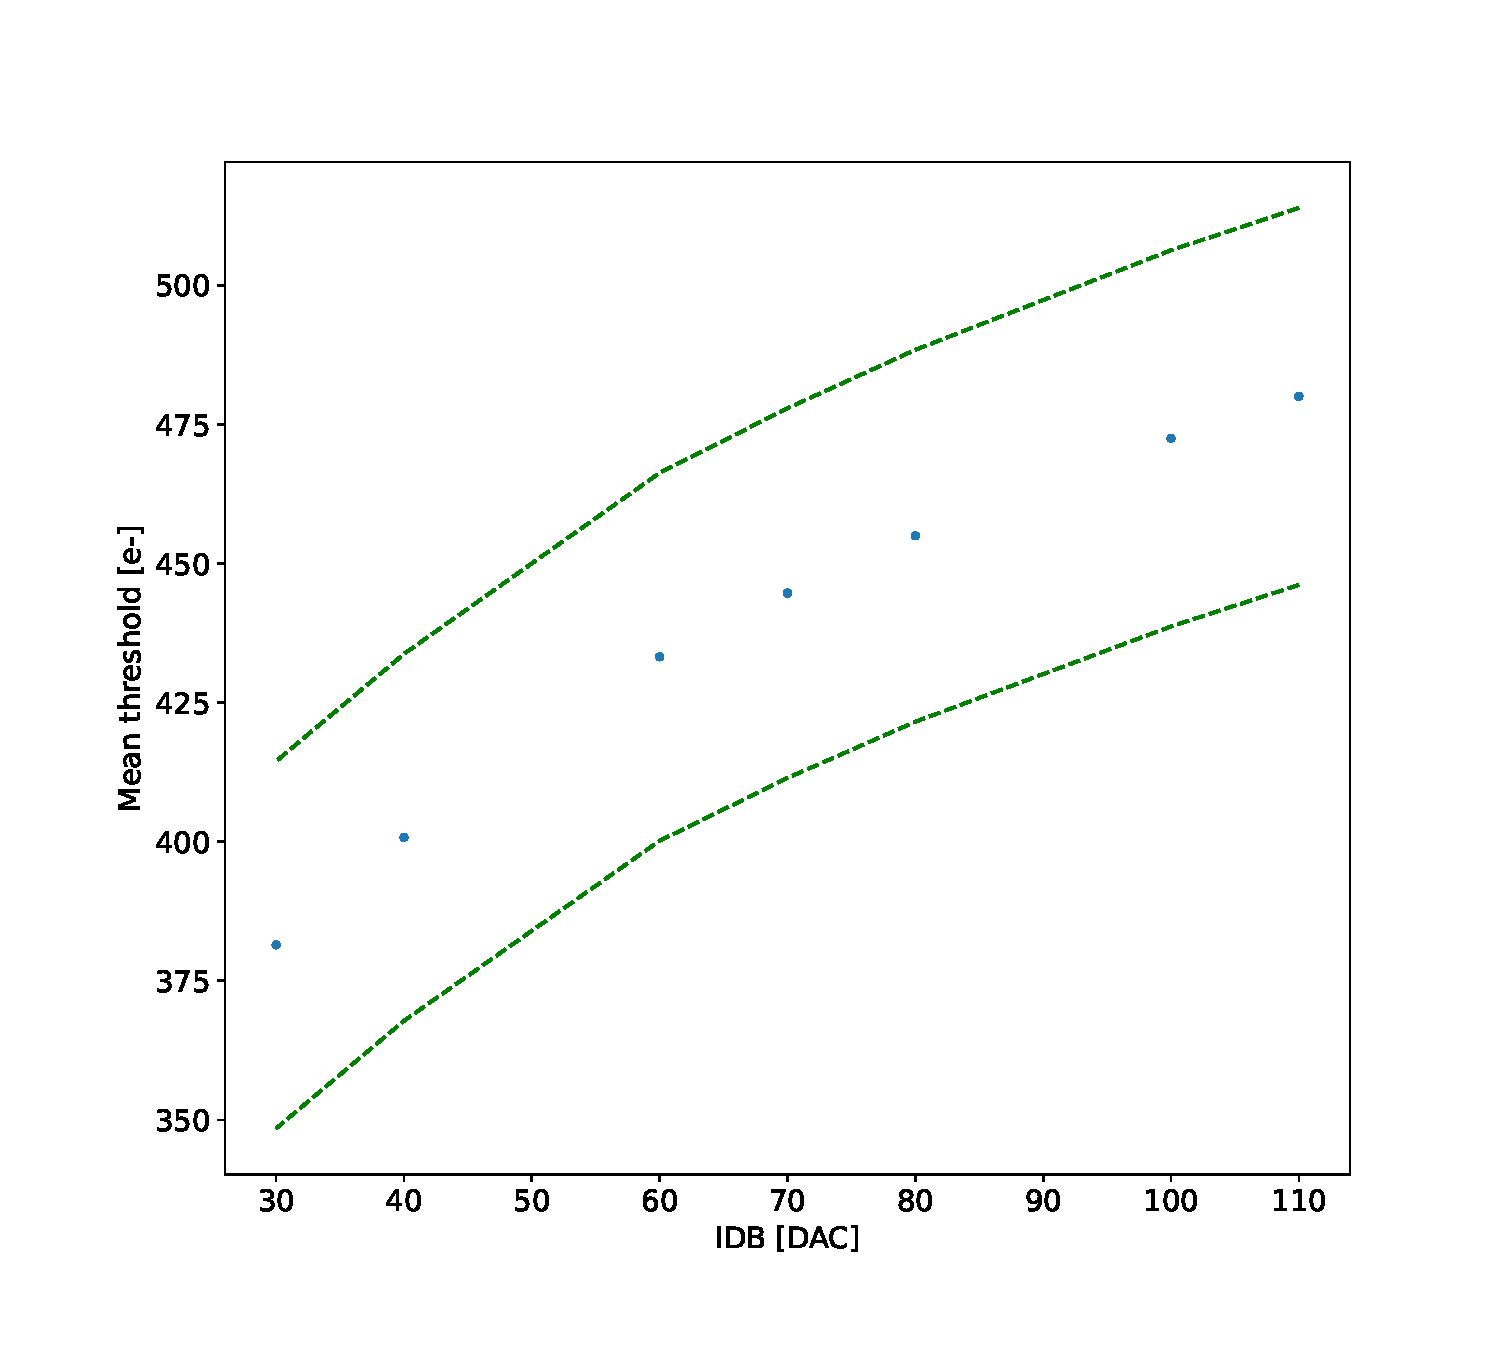
\includegraphics[width=.75\linewidth]{figures/charaterization/thr_vs_IDB.pdf}
            \caption{}
            \label{fig:threshold_vs_IDB}
        \end{figure}            
   

    \subsection{Linearity of the ToT}    
        %python3 -i acquisition_Fe55/fit_tot_single_pixel.py -f acquisition_Fe55/source_PMOSS/ per fare il fit    
        %python3 -i acquisition_Fe55/plot_tot_single_pixel.py -f acquisition_Fe55/source_PMOSS/ -fl 'gauss_line' per fare il plot di single pixel
        I have already said in chapter \ref{chap:} that TJ-Monopix1 returns an output signal  proportional to the charge released by a particle in the epitaxial layer, which is the Time over Threshold; the ToT is saved as a 6-bit variable and then has a dynamic range equal to 0-64, which corresponds to \SIrange{0}{1.6}{\us} assuming a clock frequency of \SI{40}{MHz}.
        When a pulse is longer than \SI{1.6}{\us} the counter rolls back to zero and there is no way to distinguish that charge from a lower one with the same ToT: that is the rollover of the ToT (\ref{fig:ToT_vs_charge}(a)).   

        In order to associate the ToT (in range 0-64) to the charge a calibration of the signal is necessary. It is important to keep in mind that the main application target of TJ-Monopix1 is in the inner tracker detector of HEP experiments, then the main feature is the efficiency, then a rough calibration of the signal to charge is fine; \red{this information can be used to improve??}. 
        
        The study of the output signal is made possibile via the injection: since the pulses are triangular the ToT is expected to be almost linear depending on the injection charge value.
        To verify this statement and study the deviations from linearity I've fit the ToT versus the charge injected for all pixel within the matrix.
        In figure \ref{fig:ToT_vs_charge}(b) there is an example of fit for a pixel belonging to the flavor 1, while in figure \ref{fig:ToT_histograms_all_fl} and \ref{fig:ToT_fit_param_map} there are the histograms and the maps of the parameters of the line-fit for all flavors.  

        Before performing the fit I have calculated the mean value of the ToT of the pulses recorded for each pulse amplitude and I used the mean ToT as value for the fit. 
        The aim of the calibration obviously is finding a relation only in the range 0-64 without taking into account the rolling over hits: therefore, to prevent the rollover data from reducing the mean ToT introducing a bias in the mean value, I cut and I did not consider them. 
        If a signal bigger than the \SI{1.6}{\us} is expected in the usage of the detector, the threshold must be raised or the gain reduced, making the expected output signal in range 0-64. 
        In figure \ref{fig:ToT_vs_charge} (b) are shown both the fits with a line (red) and with a second order polynomial (green): at the bounds of the ToT range values deviate from the line model. Since the deviation is low than \red{controlla quant'era, questo ha un impatto sul valore della calibrazione di tipo .. che è trascurabile al primo ordine. e comunque hai problemi ai bounds mentre al centro hai comunque una buona linearità.}. 
        \red{come mai si vede una banda? anche negli altri plot successivi sono molto evidenti.}

        \begin{figure}[h!]
            \begin{subfigure}{.5\textwidth}
            \centering
            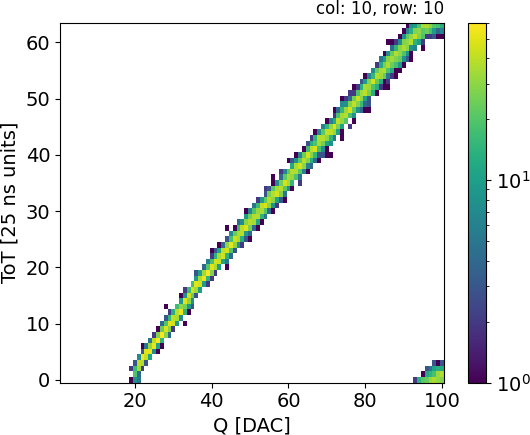
\includegraphics[width=.98\linewidth]{figures/charaterization/ToT_rollover.png}            
            \end{subfigure}
            \begin{subfigure}{.5\textwidth}
            \centering
            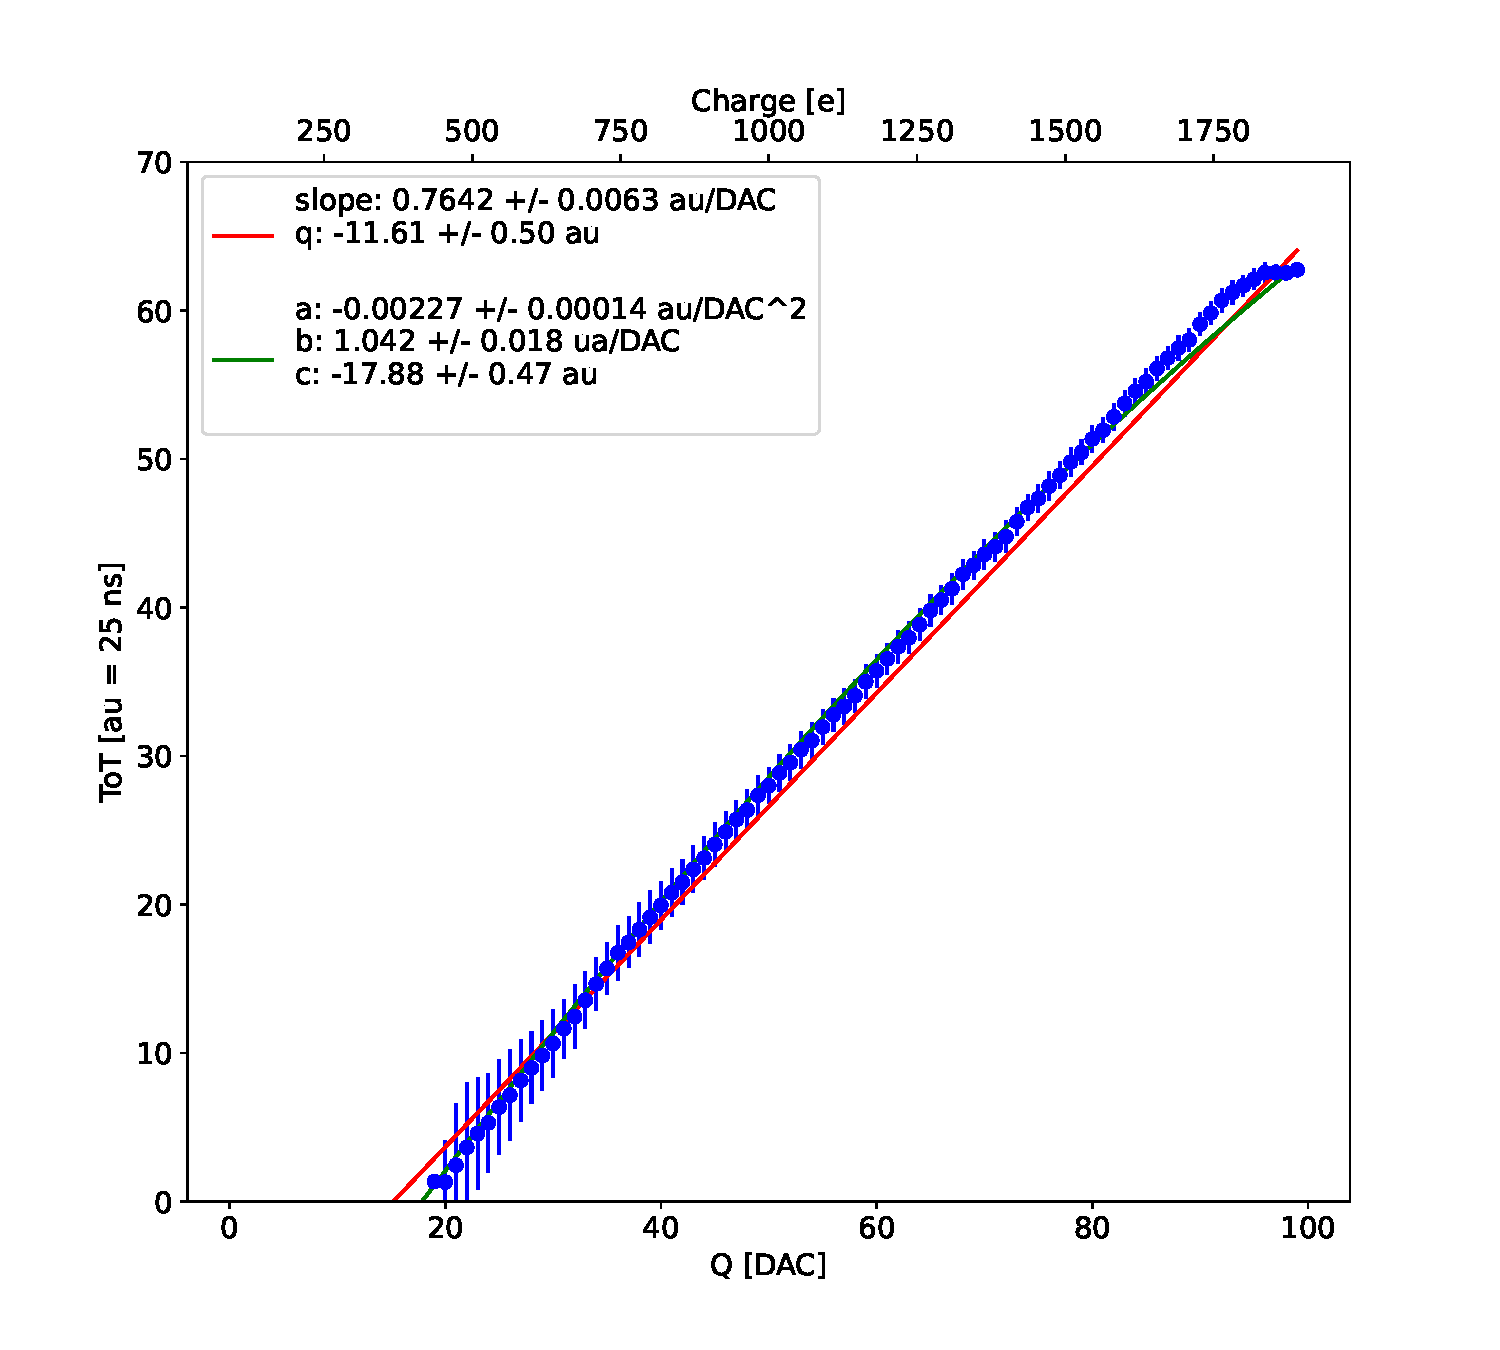
\includegraphics[width=.98\linewidth]{figures/charaterization/ToT_injection.pdf}
            \end{subfigure}
            \label{fig:ToT_vs_charge}
            \caption{The figures refer to pixel (10,10) of the PMOS-reset flavor (1). (a)Histogram of the injection pulses: the ToT is in range 0-64 since it is represented by 6 bit, so when achieving the 64 it rolls over back to the zero. (b) Mean ToT vs the the charge: the mean has been calculated cutted the rolling hits. }
        \end{figure}    

        \begin{figure}[h!]
            \begin{subfigure}{.5\textwidth}
            \centering
            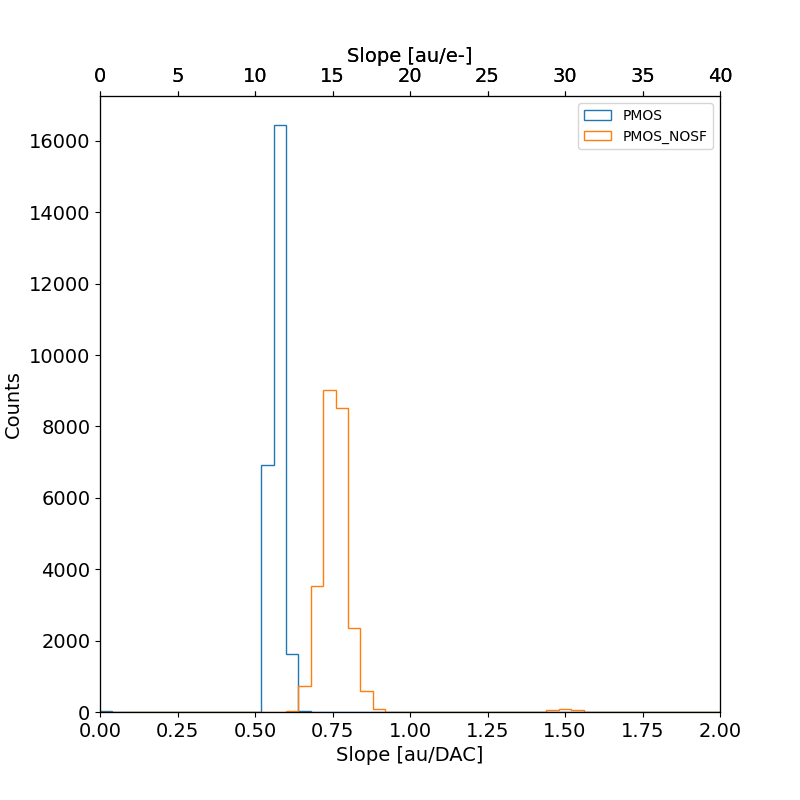
\includegraphics[width=.98\linewidth]{figures/charaterization/slope_histogram.png}
            \end{subfigure}
            \begin{subfigure}{.5\textwidth}
            \centering
            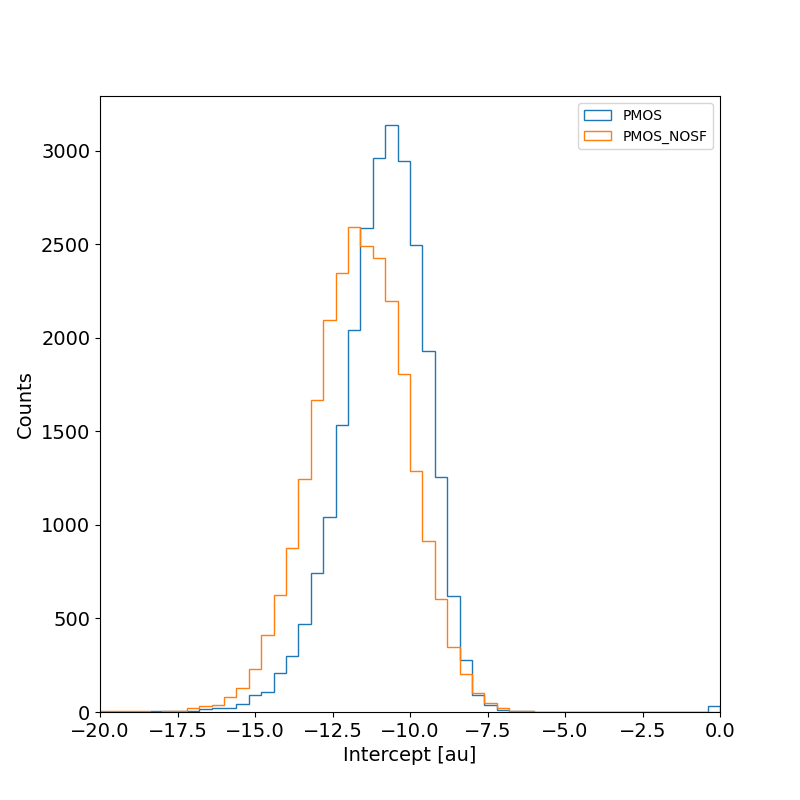
\includegraphics[width=.98\linewidth]{figures/charaterization/intercept_histogram.png}
            \end{subfigure}
            \caption{(a); (b)}
            \label{fig:ToT_histograms_all_fl}
        \end{figure} 

        \begin{figure}[h!]
            \begin{subfigure}{.5\textwidth}
            \centering
            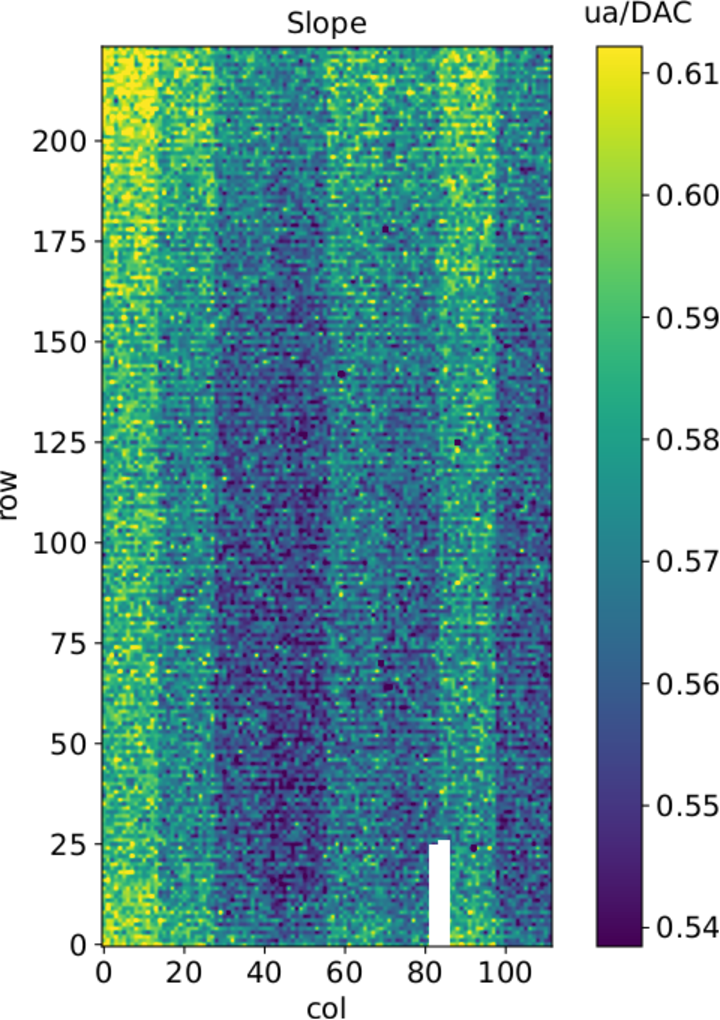
\includegraphics[width=.99\linewidth]{figures/charaterization/slope_map.pdf}
            \end{subfigure}
            \begin{subfigure}{.5\textwidth}
            \centering
            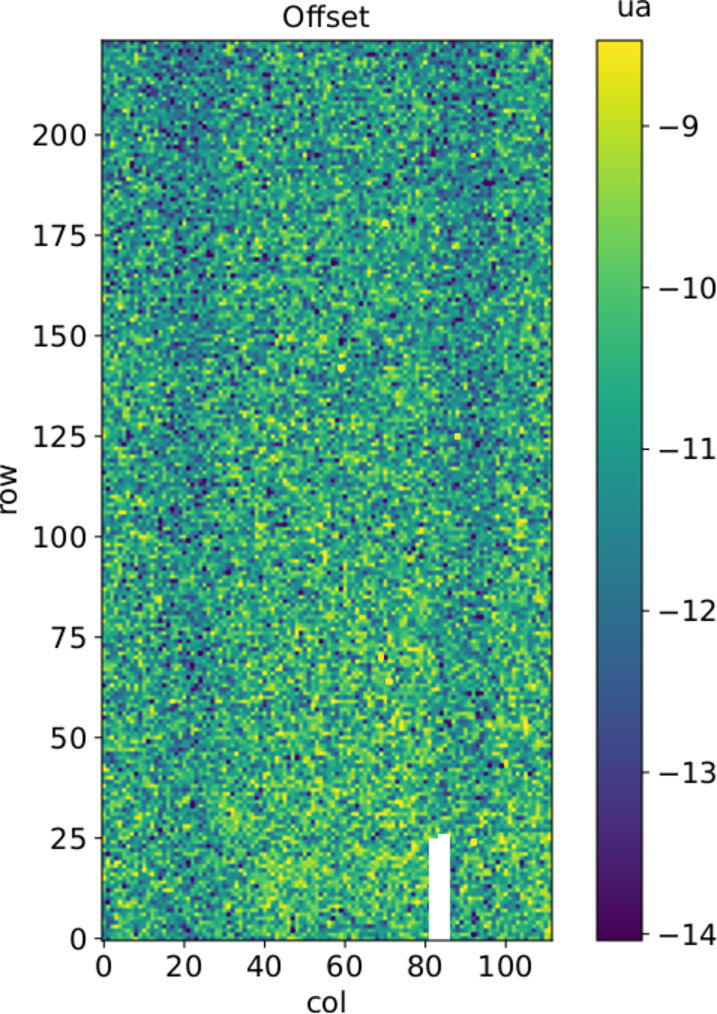
\includegraphics[width=.99\linewidth]{figures/charaterization/offset_map.pdf}
            \end{subfigure}
            \label{fig:ToT_fit_param_map}
            \caption{}
        \end{figure} 
        \red{perchè noise e th sono diverse per diversi flavor? Controlla cos' hanno di diverso.}
        \begin{table}
            \begin{center}
            \begin{tabular}{| c |  c | c | c |c |}
            \hline
            & PMOS 0 & PMOS 1 & PMOS 2 & HV \\
            \hline
            \hline
            Slope [au/DAC] & 0 .75566 $\pm$ 0.00149 & 0.57145 $\pm$ 0.00025 \\
            Slope dispersion [au/DAC] & 0.03841 $\pm$ 0.00037 & 0.01685 $\pm$ 0.00016\\
            Intercept [au] & -11.6070 $\pm$ 0.0089 & -10.824 $\pm$ 0.019 \\
            Intercept dispersion [au] & 1.5176 $\pm$ 0.0063 & 1.225 $\pm$ 0.013\\
            \hline
            \end{tabular}
            \caption{}
            \label{tab:}
            \end{center}
        \end{table}        

        \subsection{Calibration of the ToT}
        %python3 -i acquisition_Fe55/fit_tot_single_pixel.py -f acquisition_Fe55/source_PMOSS/Fe_acquisitions_6V/ per fare i fit. Attenzione che prende i file degli istogrammi npz già
        Considering that the charge injected in the FE goes to fill capacitor which is different from pixel to pixel, the true charge injected does not correspond to what expected assuming C equal to \SI{230}{aF}, the nominal value. 
        Accordingly to that, a verification of the value provided and an absolute calibration of this capacity is needed to have a correspondence of the signal in electrons. 

        For this pourpose a Fe55 radioactive source has been employed; the Fe55 is en extremely important radionuclide in the calibration of X-ray spectrometers, proportional counter and scintillator detector. It emits two X-photons during the electron capture decay: the first one (K$_\alpha$) at \SI{5.9}{keV} and the second one (K$_\beta$) at \SI{6.5}{keV}.
        The K$_\alpha$ photon, which does photoelectric effect in the silicum, has an absorption length $\lambda$=\SIrange{7}{8}{\um}, and the probability of being assorbed in the \SI{25}{\um} thick epitaxyal layer is $\sim$0.95\%.
        The electron emitted has an energy equal to the photon one, so recalling that the mean energy needed to produce a couple electron-vacuum is \SI{3.65}{eV}, the signal produced by the Fe55 source is expected to be \SI{1616}{e-}.
        In figures \ref{fig:} and \ref{fig:} are shown two histograms of the ToT spectrum of the Fe55 source for two different pixels. The peak corresponds to the events with completely absorption of the charge produced in the depleted region, while the long tail on the left to all the events with partial absorption due to charge sharing among neighbors pixels. 
        In order to reduce the charge sharing and reducing the tail on the left, the pixel dimension in TJ-Monopix2 has been reduced down to \red{check}. 
        Looking at the histograms for pixel () and () a significant difference in the peak to tail ratio leaps out. 
        This difference in the efficiency of detecting the signal can be related with the position of the pixel in the matrix: in particular pixels in the upper part of the matrix (rows 112-224) have a more prominent peak, while in pixels in the lower part (rows 0-111) there is a higher partial absorption. 
        I recall now that there is a slighly difference in the structure of the low dose-epi layer (\ref{chap:}) among the rows in the matrix, in particular pixels in rows 112-224 are supposed to have a higher efficiency in the pixel corner. 
        
        For the calibration I have need to establish the peak position; to do that I perform a fit of the ToT histogram of each pixels. As fit functions I test both the solutions below:  
        \begin{equation}
            f(x, N, \mu, \sigma) = \frac{N}{\sigma \sqrt{2\pi}} e^{-\frac{1}{2}(\frac{(x-\mu)}{\sigma})^2}
        \end{equation} 

        \begin{equation}
            f(x, m, q, N, \mu, \sigma) = m\,x + q + \frac{N}{\sigma \sqrt{2\pi}} e^{-\frac{1}{2}(\frac{(x-\mu)}{\sigma})^2}
        \end{equation}          
        
        Nel primo caso ho fittato pochi pixel attorno a picco: il range è stato determinato .. controlla. 
        Nel secondo caso invece il range è..
        
        \begin{figure}[h!]
            \begin{subfigure}{.5\textwidth}
            \centering
            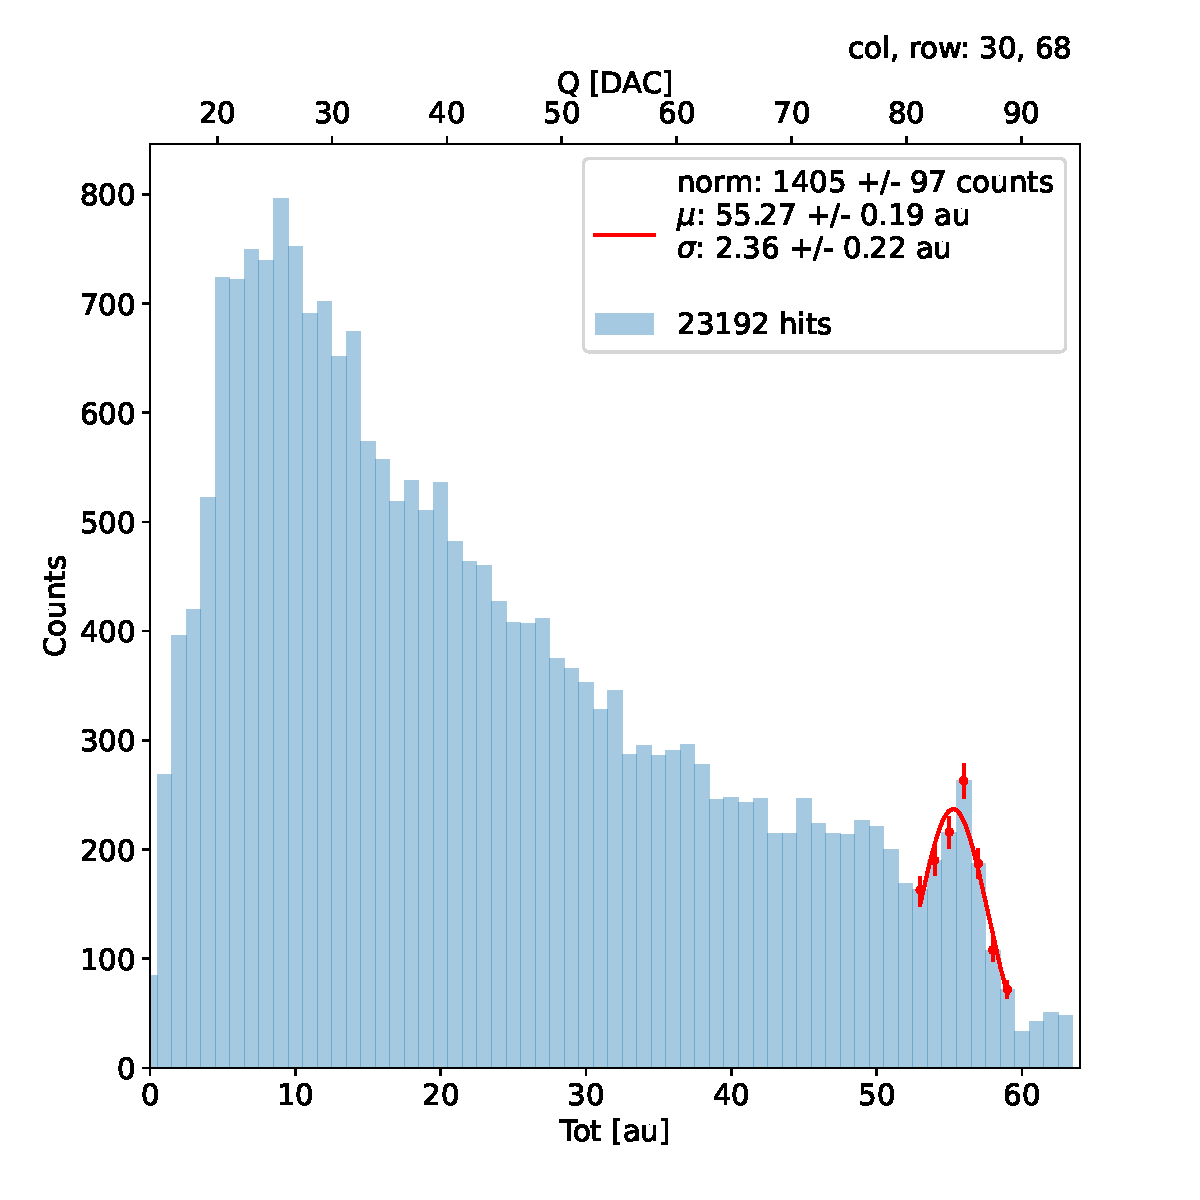
\includegraphics[width=.99\linewidth]{figures/charaterization/fit_gauss_r69.pdf}
            \label{fig:}
            \end{subfigure}
            \begin{subfigure}{.5\textwidth}
            \centering
            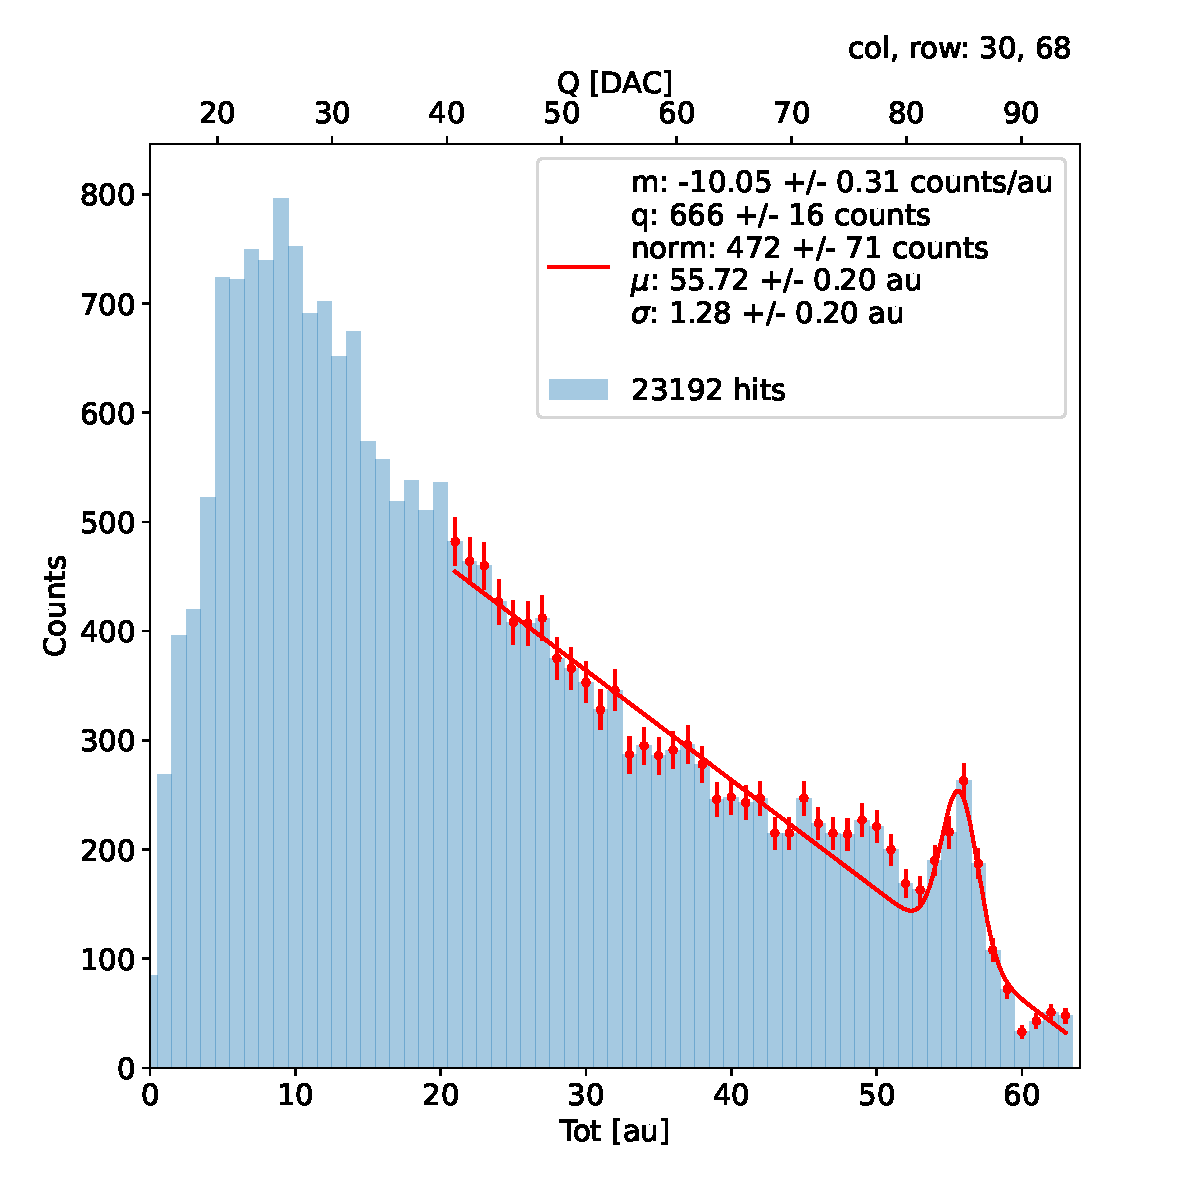
\includegraphics[width=.99\linewidth]{figures/charaterization/fit_line_gauss_r69.pdf}
            \label{fig:}
            \end{subfigure}
            \caption{due pixel per far vedere la differenza tra i fit. Sottolinea che in rosso ci sono i bin fittati. La doppia scala utilizza le info trovate nel paragrafo precedente per il dato pixel in questione. Per avere una corrispondenza grezza in elettroni basta moltiplicare per 20 e- dac. }
        \end{figure}            

        \begin{figure}[h!]
            \begin{subfigure}{.5\textwidth}
            \centering
            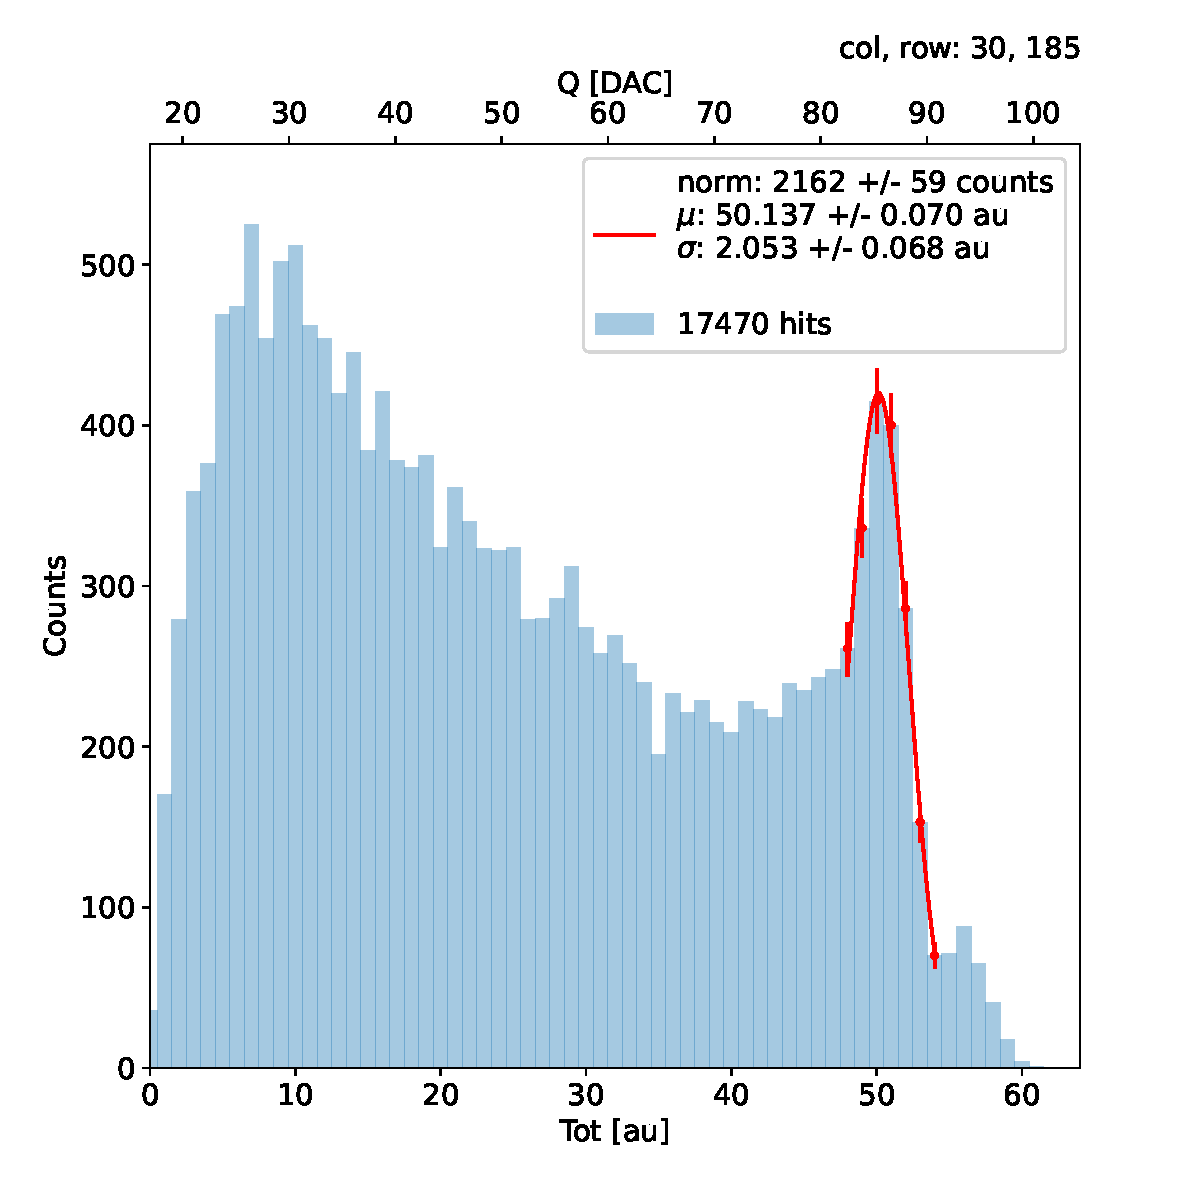
\includegraphics[width=.99\linewidth]{figures/charaterization/fit_gauss_r185.pdf}
            \label{fig:}
            \end{subfigure}
            \begin{subfigure}{.5\textwidth}
            \centering
            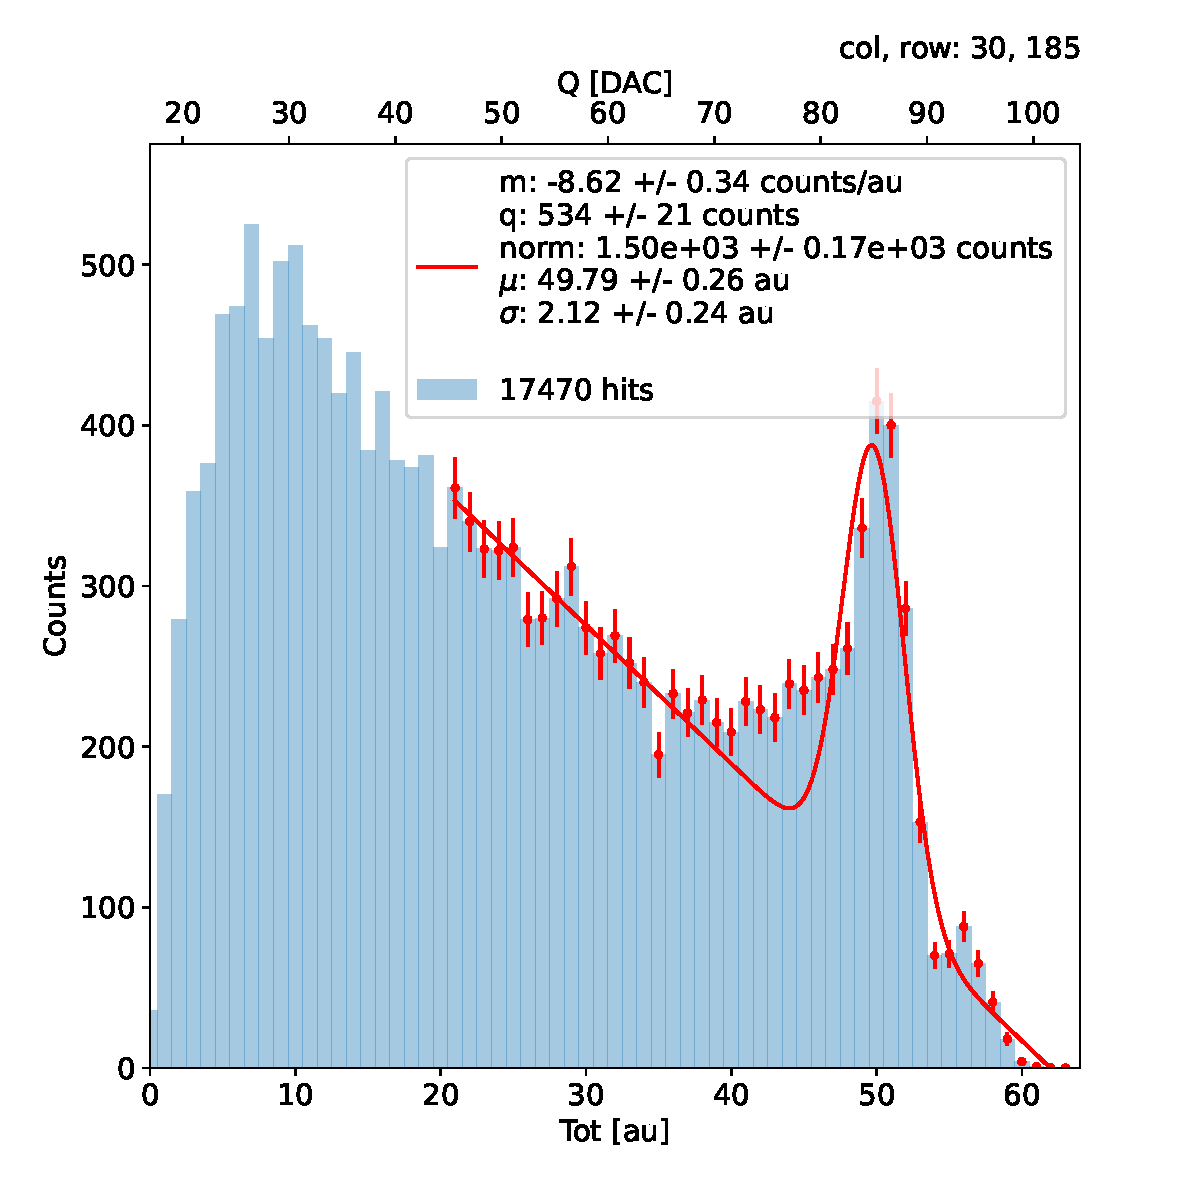
\includegraphics[width=.99\linewidth]{figures/charaterization/fit_line_gauss_r185.pdf}
            \label{fig:}
            \end{subfigure}
            \caption{due pixel per far vedere la differenza tra i fit}
        \end{figure}    
        
        Sebbene non molto significativa trattandosi di una differnza minore di 0.5 /64  per cento, la differenza della quantità di coda rispetto al picco tra le due parti della amtrice introduce una differenza e un effetto sistematico nel fit che dipende da quale funzione di fit sia meglio per fittare. 
        Volendo utilizzare un criterio empirico per stabilire il fit più buono sappiamo che il acso di assorbimento totale del fotone è dovrebbe essere il valore più spostato a destra (esclusi i dati del fotone kbeta) e il cui valore si usa per la calibrazione. 
        Un modo quindi per aveere un fit che non risente di questo sistematico potrebbe essere usare un algoritmo di search edge. 
        
        Un modo per valutare invece la bontà dei due fit potrebbe essere guardare la variabile chi2. Per rendere confrontabili i due valori però  bisogna calcolare la variabile sul solito interllavot di fit, determinato quindi dal fit con ggaussiana singola. 
        Sottraggo i chi2 e plottO: dove la mappa ha valori positivi allora ho un fit gauss migliroe, ecc. 
        With the gaussian fit $\sim$ 80 pixels, while with the sum gaussian and the line sim 1000. 
        \begin{figure}[h!]
            \begin{subfigure}{.5\textwidth}
            \centering
            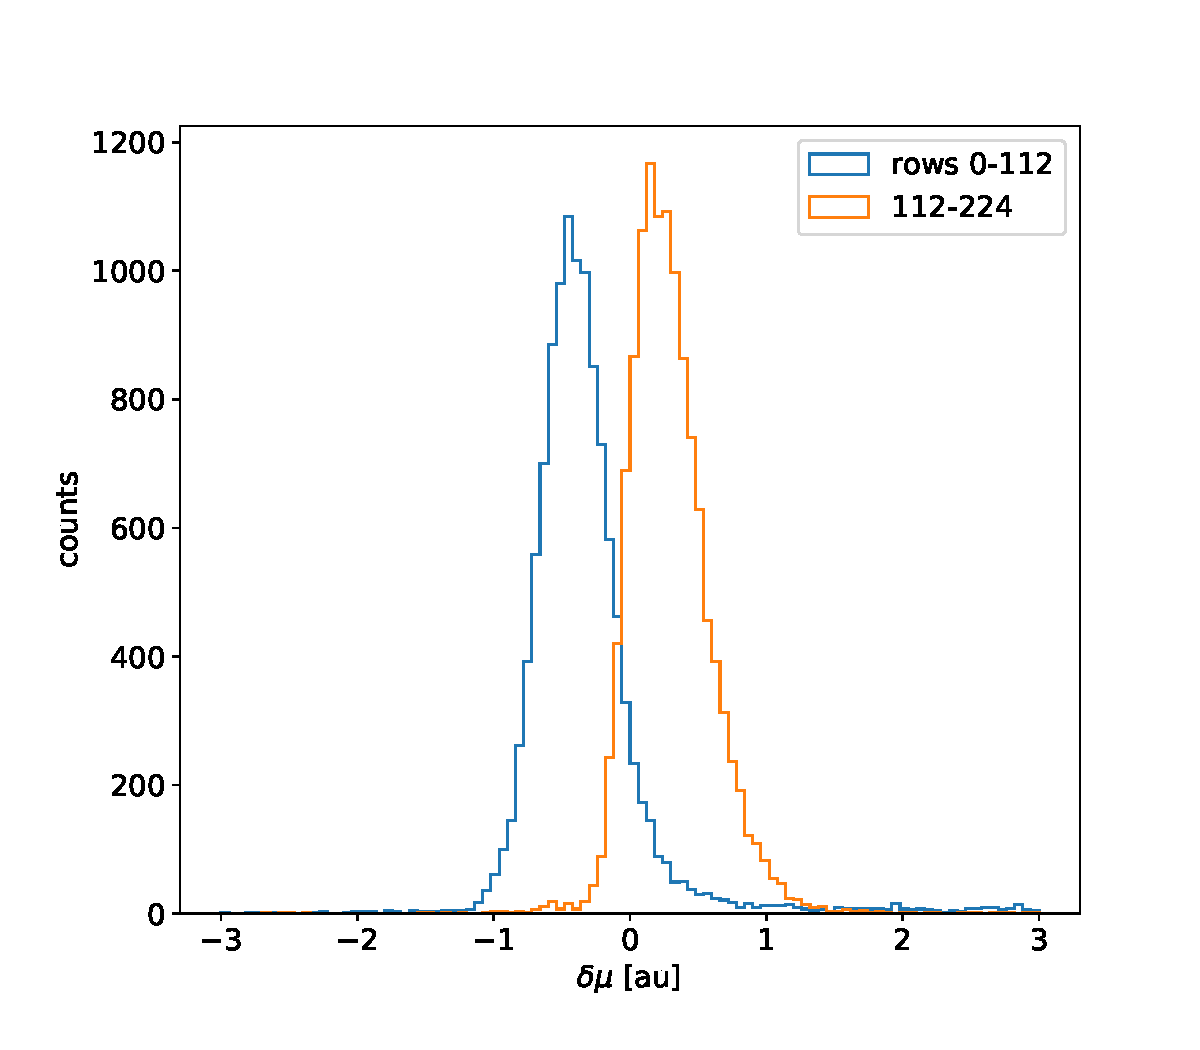
\includegraphics[width=.99\linewidth]{figures/charaterization/deltam_Fe.pdf}
            \label{fig:}
            \end{subfigure}
            \begin{subfigure}{.5\textwidth}
            \centering
            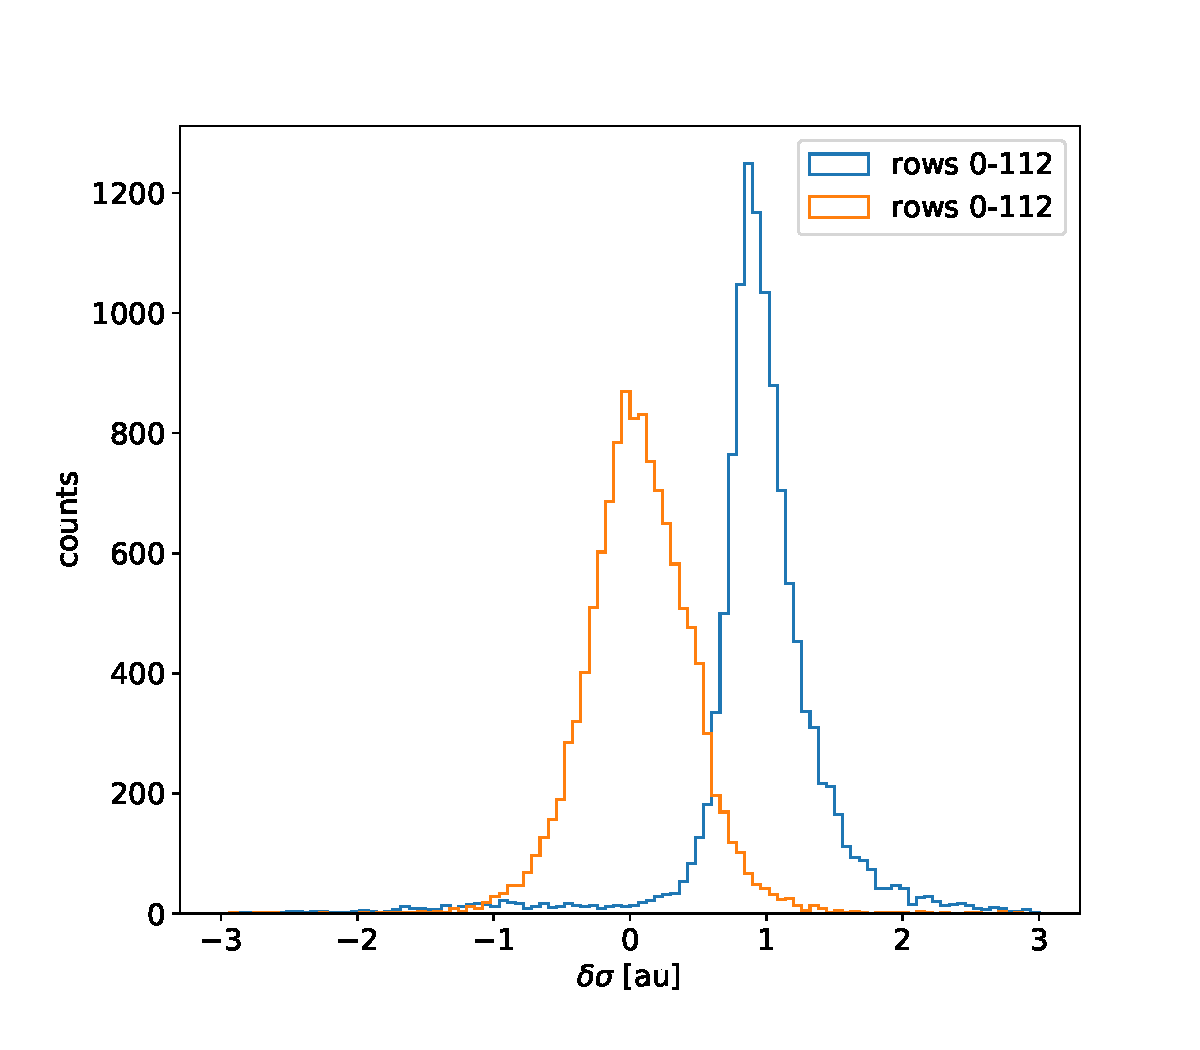
\includegraphics[width=.99\linewidth]{figures/charaterization/deltas_Fe.pdf}
            \label{fig:}
            \end{subfigure}
            \caption{}
        \end{figure}            

        \begin{figure}[h!]
            \centering
            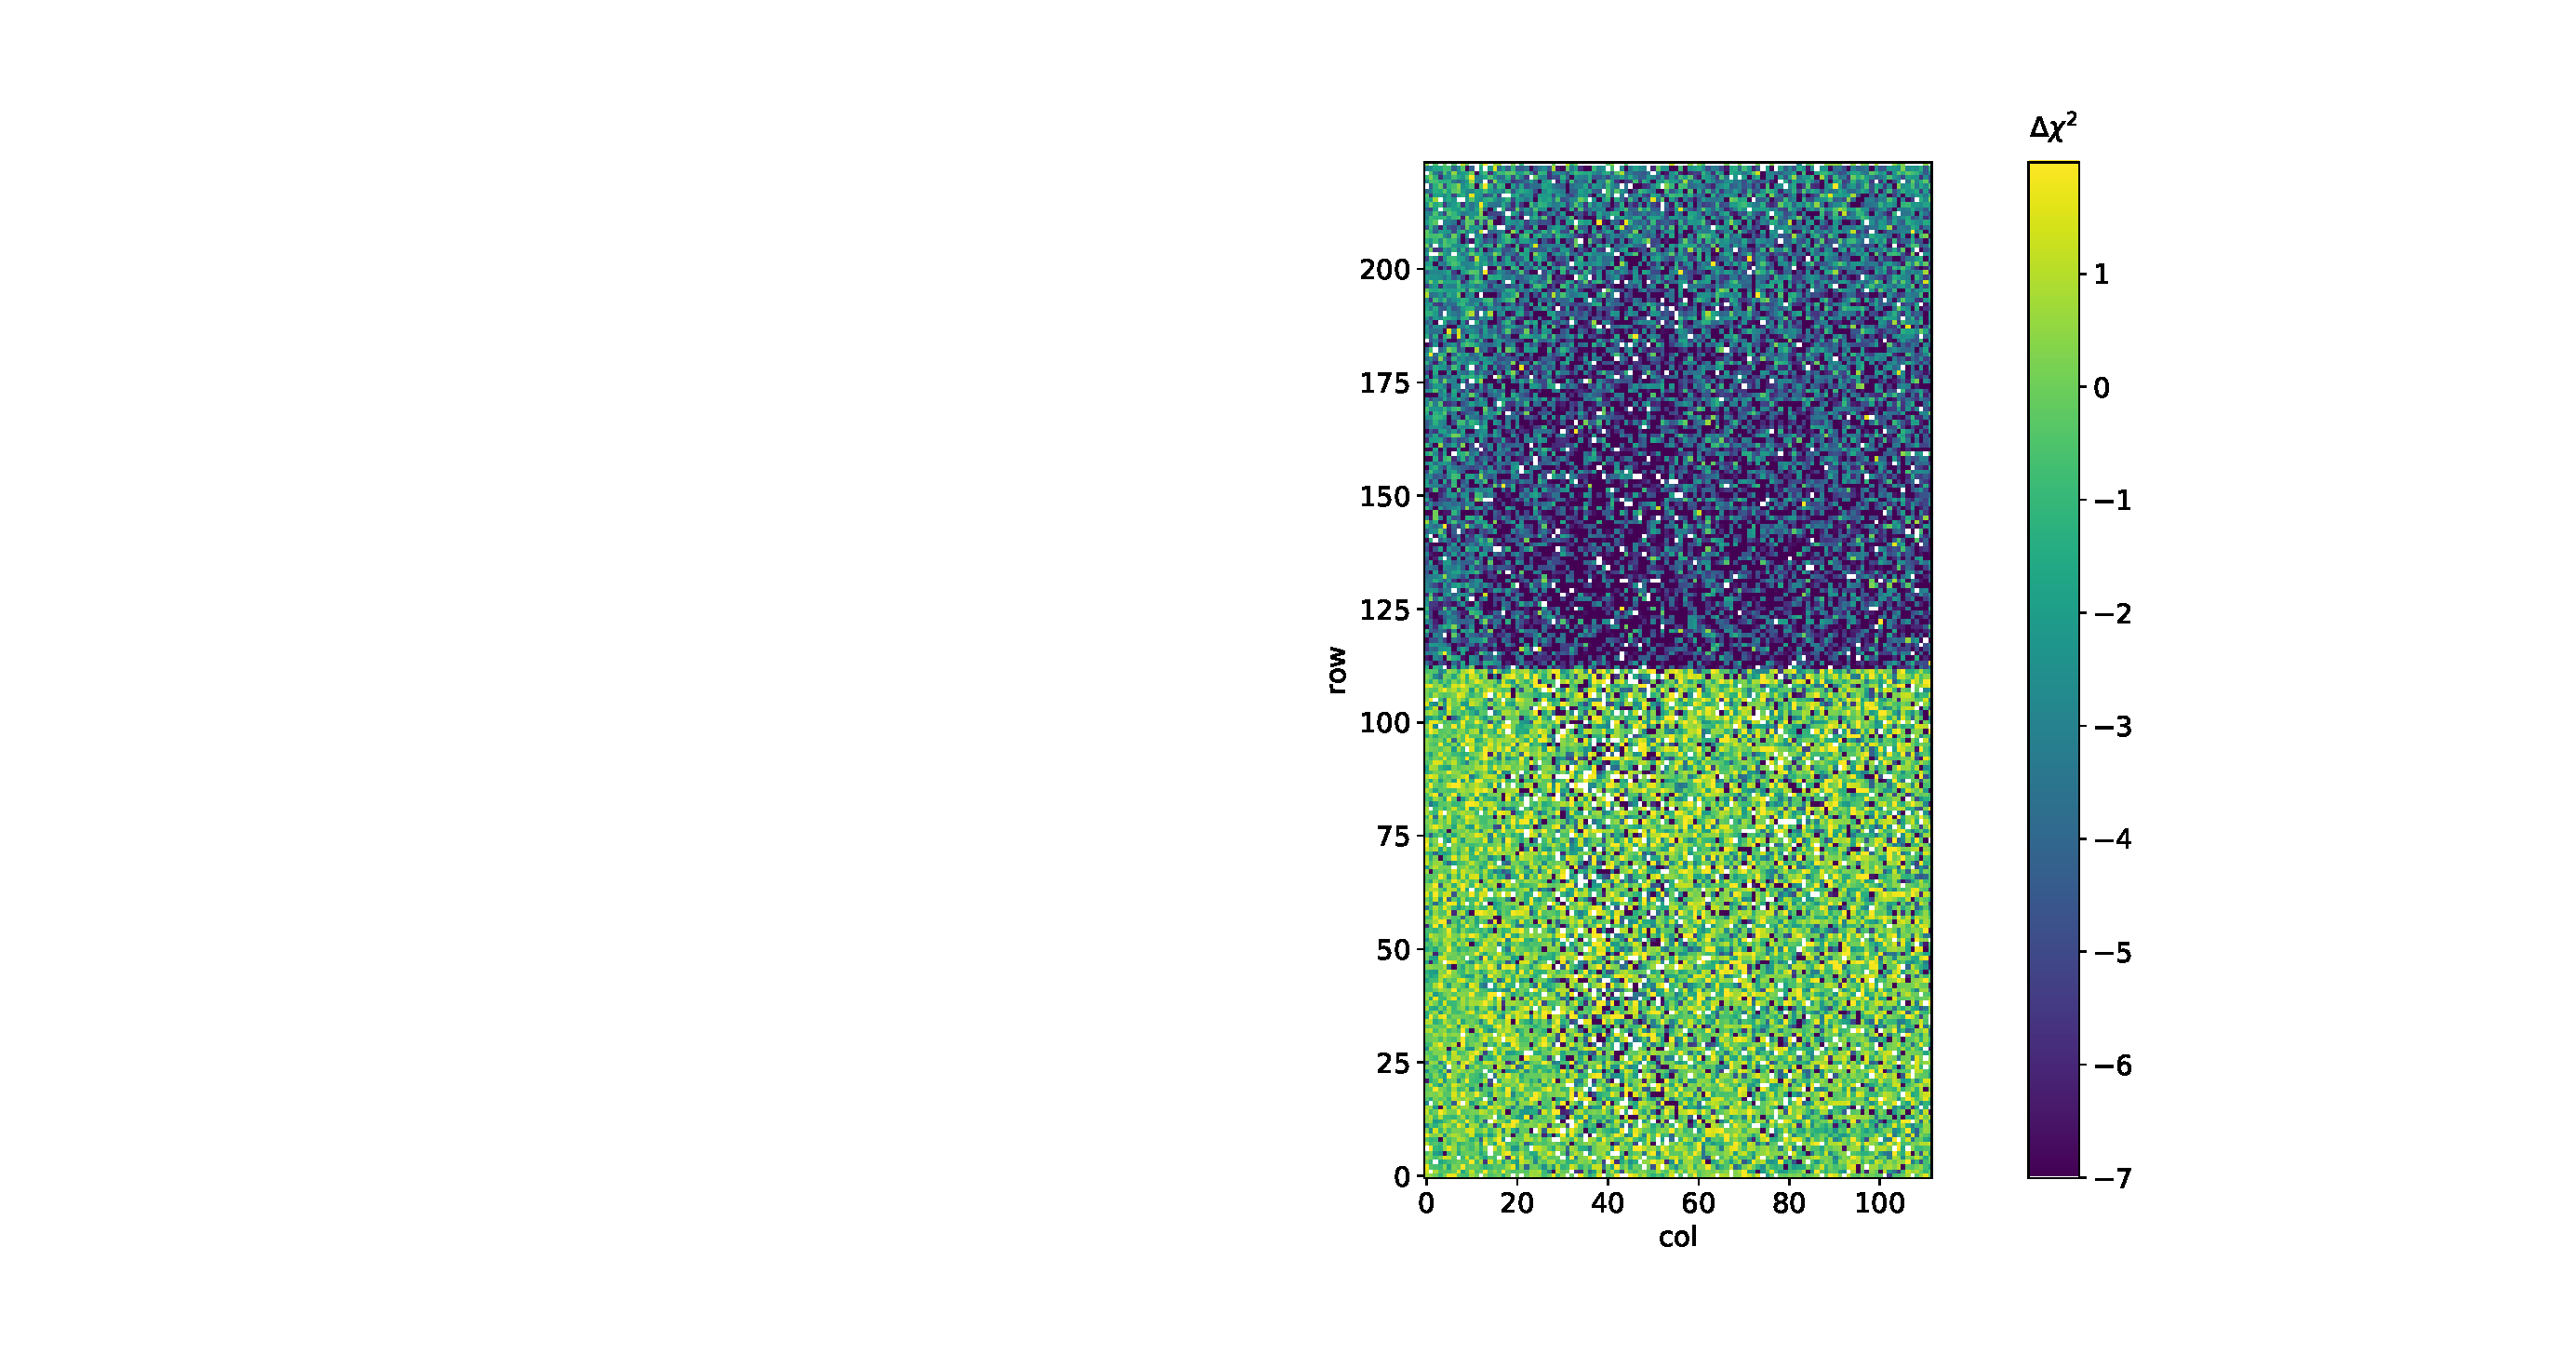
\includegraphics[width=.90\linewidth]{figures/charaterization/deltachi2_Fe.pdf}
            \caption{}
            \label{fig:chi2_map}
        \end{figure}            

        
    
     
     
     \subsection{Measurements with radioactive sources}
        %python3 -i acquisition_Fe55/find_cluster.py -d acquisition_Fe55/source_PMOSS/noise_acquisitions_6V -> per cluster dimension e spettro del noise
        %python3 -i acquisition_Fe55/hit_map.py -f acquisition_Fe55/source_PMOSS/2022-04-07/2022-04-07_10-10-01_acq.h5 -> per le hit map, comprese qualche hitmap dei cluster
        %python3 -i acquisition_Fe55/Sr90_spectrum.py -d acquisition_Fe55/source_PMOSS/noise_acquisitions_6V/ -> per fare i plot dello stronzio
        Signal response characterization using radioactive sources 
        \red{CI metterei i plot con ferro, stronzio e cosmici, pag 55 tesi M}
        ToT con doppia scala (calibrata in elettroni e non in ToT)
         hit per cluster
         dimensione cluster
         hit map di un paio di tracce?

    \subsection{Fe vs bias}
         \begin{itemize}
             \item rate vs bias 
             \item posizione del picco del ferro vs bias    
             \item eventi sotto il picco vs eventi nella coda
         \end{itemize} 
         
    \subsection{Dead time measurements}
        The hit loss is due to analog and digital pile up: the first one occurs when a new hit arrives during the pre-amplifier response, the second instead, which is the more relevant contribution with high rate, while the information of the previous hit has not yet been transferred to the periphery.  
        As only one hit at a time can be stored on the pixel's RAM, until the data have completed the path to get out, the pixel is paralyzed and the dead time $\tau$ almost corresponds with the time needed to trasmit the data-packets off-chip.
        Since the exportation of data from pixel to the EoC occurs via a 21-bits data bus, only one clock cycle is need to transfer the data to the end of column and the dead time bottleneck is given by the bandwidth of the serializer at the EoC. In our setup the serializer operates at 40 MHz, thus to transmit a data packet (27-bit considering the addition at the EoC) at least \SI{675}{ns} are needed. 
        For what we have said so far, the R/O is completely sequential and therefore is expected a linear dependence of the reading time on the number of pixels to read:
        \begin{equation}
            \tau =\, 25\: \unit{ns}\, \times\, (\alpha\, N +\, \beta)
            \label{eq:reading_time}
        \end{equation}
        where $\alpha$ and $\beta$ are parameters dependent on the readout chain setting. 
        
        To measure and test the linearity of the reading time with the number of pixels firing, I have used the injection mode available on the chip. 
        Indeed, the injection mode allows fixing not only the amplitude of the pulse, which corresponds to the charge in DAC units, but also the period and the width.
        I have injected a fix number of pulses (100) and looked for the rate when the efficiency decreases. 
        Moreover to test that there is no dependece of the digital readout time from the charge of the pulse, I have try to change the amplitude of the pulse injected, but the parameters found were consistent with the default configuration ones.

        \red{Al posto degli esempi con 5 e 10 pixels metterei un esempio dell'efficienza vs il periodo quando leggo un singolo pixel. Una cosa che volevo fare era anche provare a fittare la slope con cui l'efficienza scende: se la slope è uguale per tutti il readout diventa completamente predittivo. }
        \begin{figure}[h!]
            \begin{subfigure}{.5\textwidth}
            \centering
            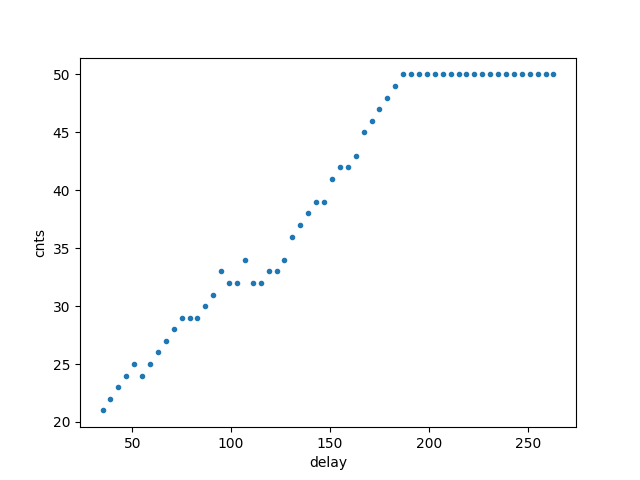
\includegraphics[width=.98\linewidth]{figures/charaterization/efficiency_5pixels.png}
            \caption{\red{efficiency vs DELAY 5 pixels}}
            \label{fig:}
            \end{subfigure}
            \begin{subfigure}{.5\textwidth}
            \centering
            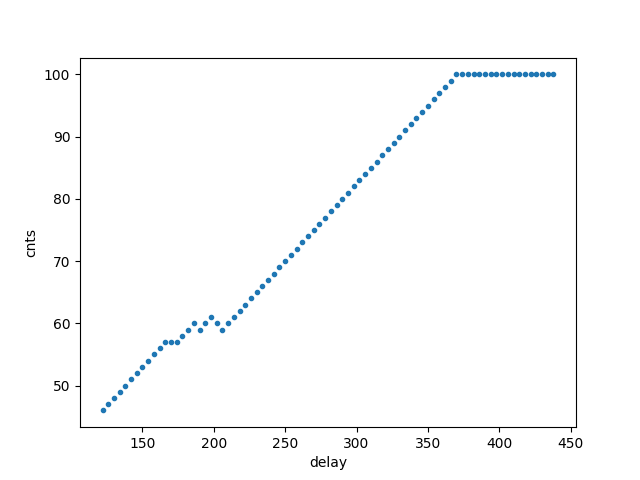
\includegraphics[width=.98\linewidth]{figures/charaterization/efficiency_10pixels.png}
            \caption{\red{efficiency vs DELAY per 10pixels}}
            \label{fig:}
            \end{subfigure}
        \end{figure}
        
        While the single pixel reading time and the dead time do not depend on the position on the pixel matrix and are equal to \red{106 (46+60)} clock counts within 1 clock count, on the other hand the $\tau$ depends on the pixel position on the matrix when more than one pixel are firing. 
        In particular the priority chain goes from row 224 to row 0, and from col 0 to 112, that means the last pixels to be read is the one on le bottom right corner of the matrix. 

        In figure \ref{fig:dead_time} is reported the reading time versus the number of pixels injected; the R/O parameters that control the reading time and their default values are reported on table \ref{tab:tab:R/O_param}.
        \begin{table}
            \begin{center}
            \begin{tabular}{|c | c | c |}
            \hline
            Parameter & Value [\si{DAC}] & Value [\si{\us}]\\
            \hline
            \hline
            START\_FREEZE & 64 & 1.6\\
            STOP\_FREEZE & 100 & 2.5\\
            START\_READ & 66 & 1.65\\
            STOP\_READ & 68 & 1.7\\
            \hline
            \end{tabular}
            \caption{Default configuation of the R/O parameters}
            \label{tab:R/O_param}
            \end{center}
        \end{table}

        The factor $\alpha$, referring to eq. \ref{eq:reading_time} is proportional to the difference (STOP\_FREEZE - START\_READ), while the offset $\beta$ lies between 5 and 15 clock counts.
        Since through the injection a random hit rate on the matrix can't be simulated, as the coordinates of the pixels to inject must be specified, for convenience I used the pixels on the same column/row. No difference in the $\alpha$ and $\beta$ coefficients has been observed between the two case. 
        \begin{figure}[h!]
            \centering
            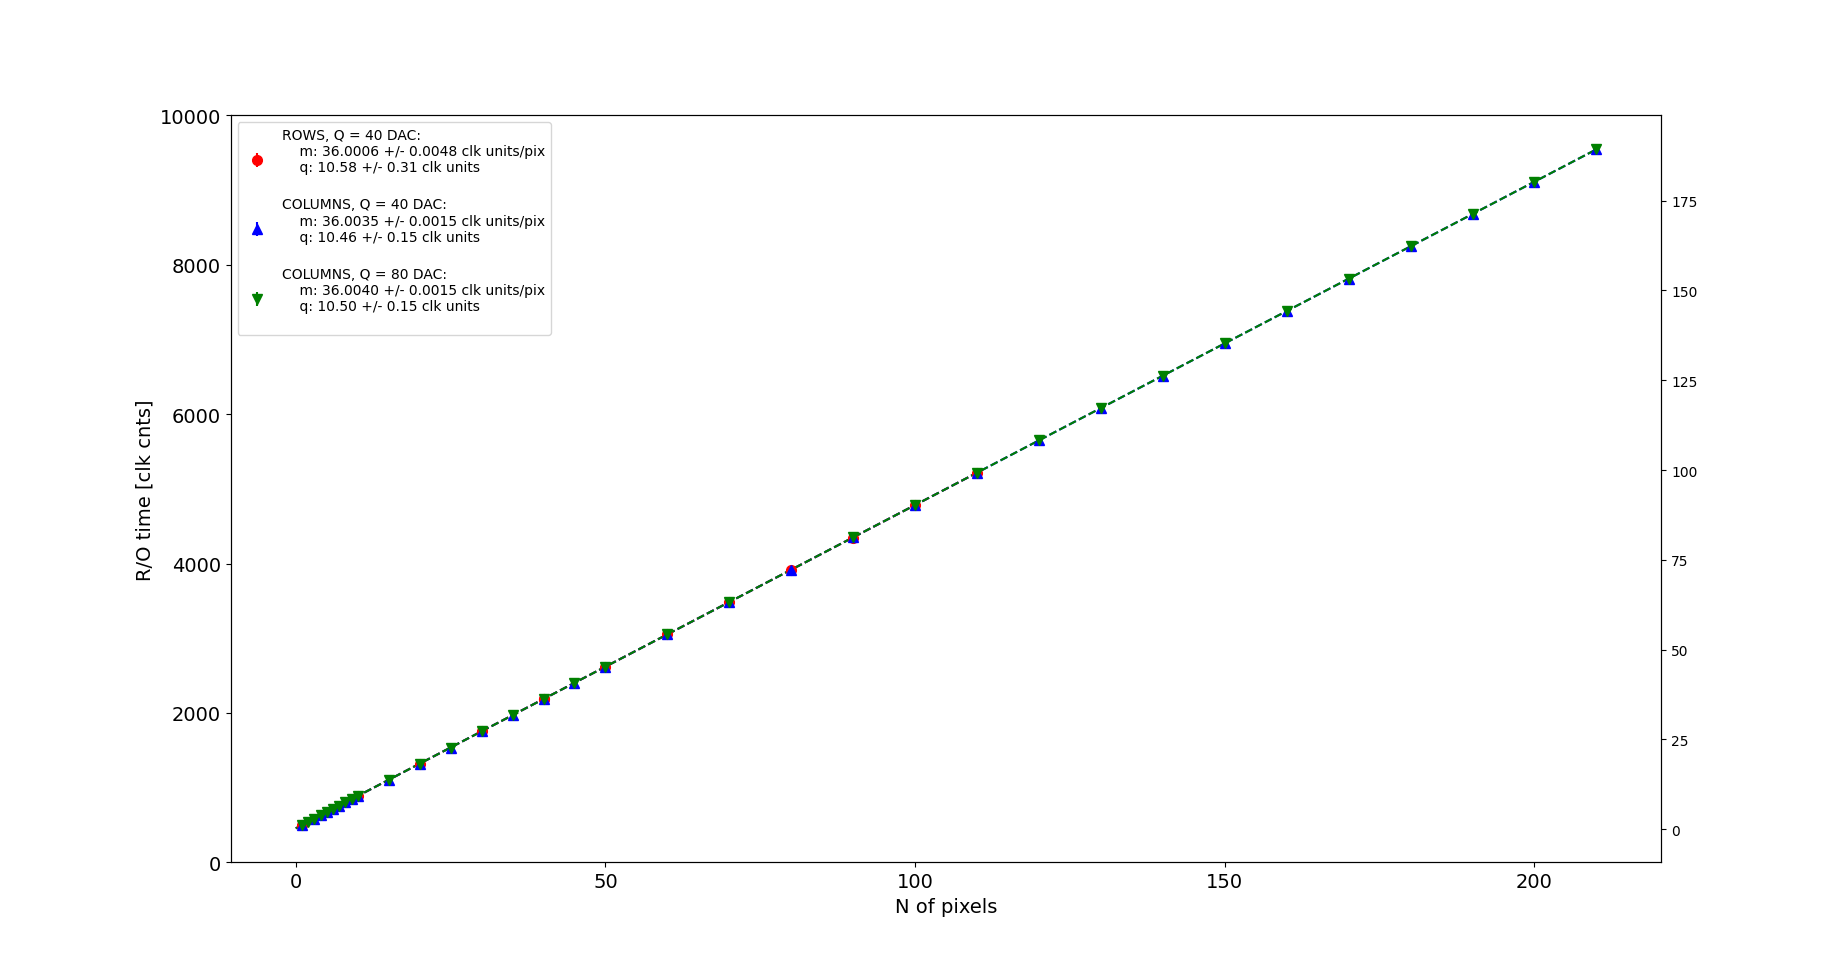
\includegraphics[width=.9\linewidth]{figures/charaterization/default_line.png}
            \caption{}
            \label{fig:dead_time}
        \end{figure}

        \begin{figure}[h!]
            \centering
            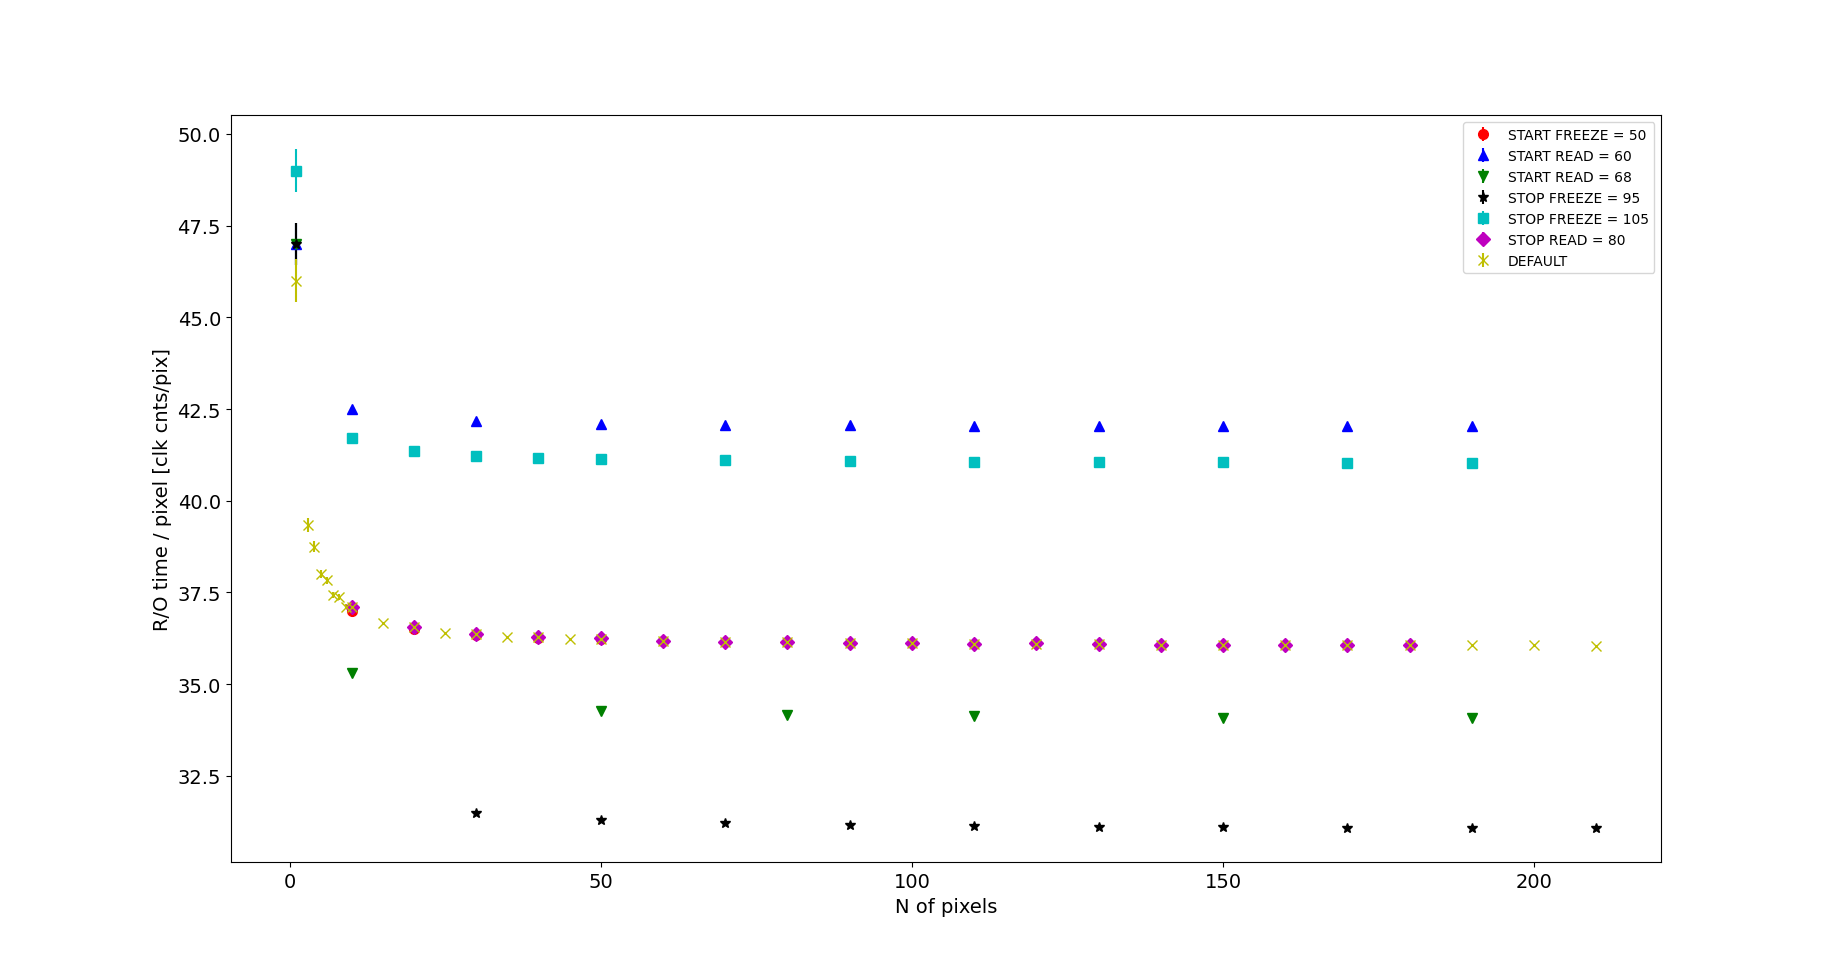
\includegraphics[width=.9\linewidth]{figures/charaterization/parameters_points.png}
            \caption{}
            \label{fig:dead_time}
        \end{figure}        

        \red{Ci sarebbe da spiegare perchè i parametri che usiamo noi come default non sono quelli che minimizzano il tempo di lettura. La spiegazione è che "Abbiamo copiato i valori dal repositorio di quelli di Bonn". Un'altra domanda potrebbe essere: come mai non ho esplorato una zona più vasta per i parametri del R/O. Cambiando molto i parametri del R/O la lettura non funzionava per niente: ad esempio CONF\_STOP\_FREEZE non può essere impostato nè sopra 105 nè sotto 95}



\section{ARCADIA-MD1 characterization}
